% !TeX root = ../content.tex
\section{轉換核心性質：Q1 與 Q2 證明}
\label{sec:kernel-properties}

\begin{figure}[H]
  \centering
  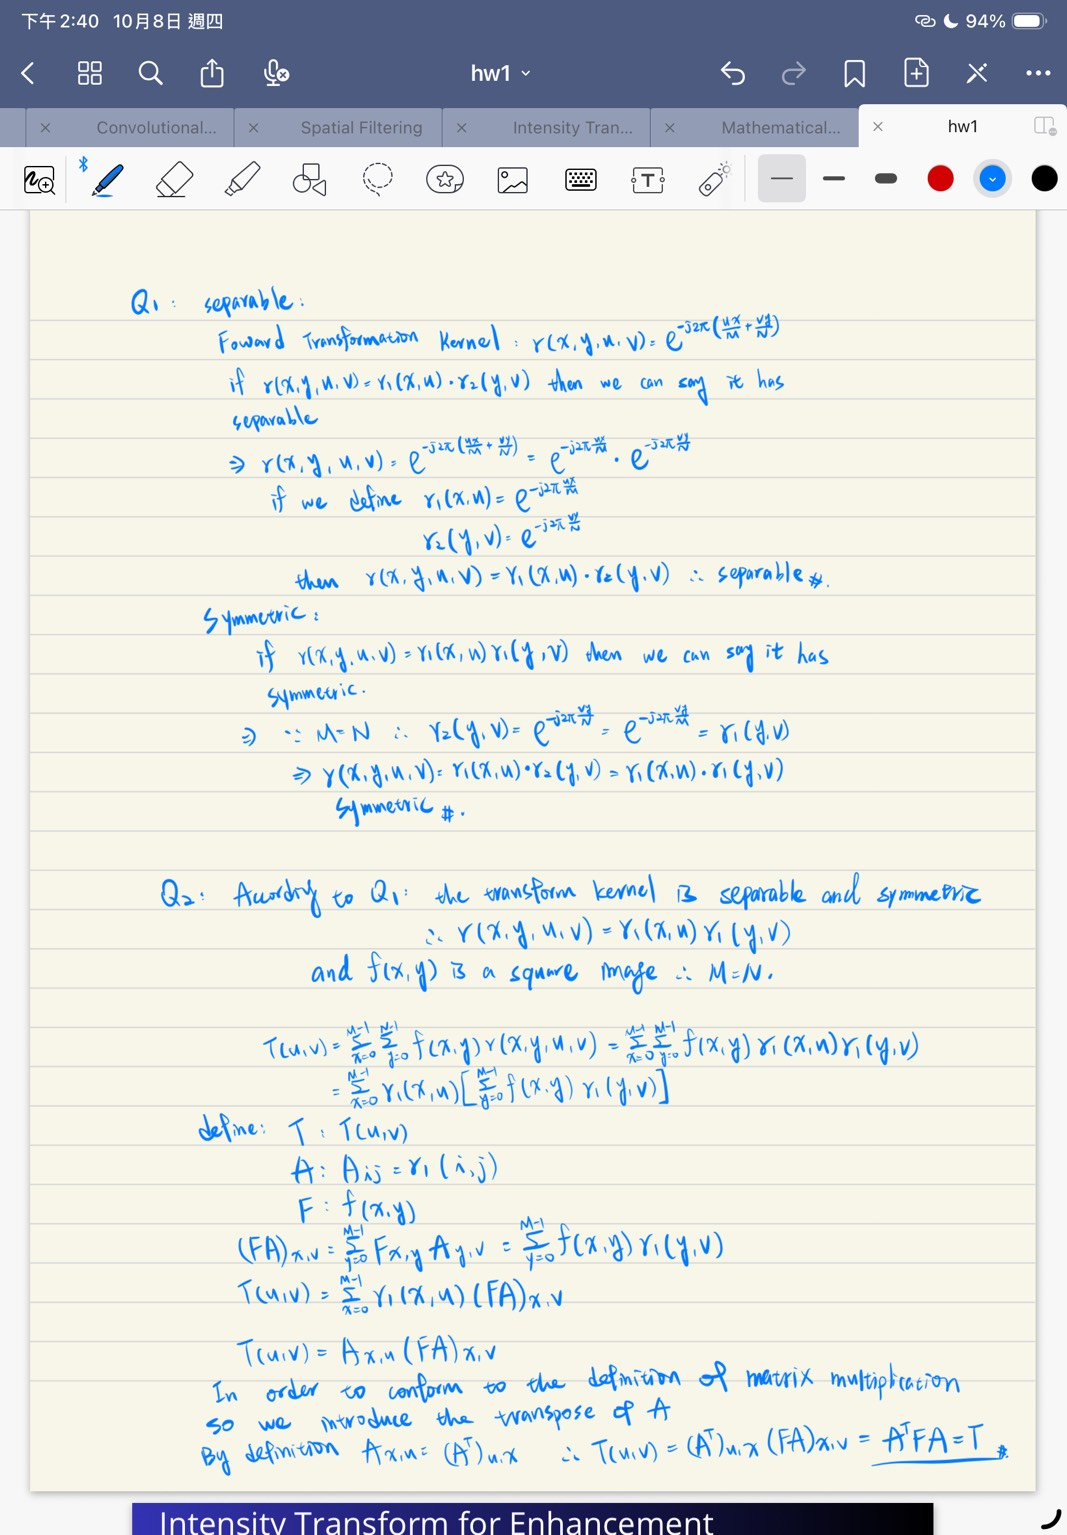
\includegraphics[width=\textwidth,height=0.70\textheight,keepaspectratio]{report_sections/Q1Q2.jpg}
  \caption{Q1 與 Q2 的手寫證明原稿。}
  \label{fig:q1q2-handwritten}
\end{figure}

\clearpage
\section{ 強度轉換 ：Gamma 處理前後比較}
\label{sec:gamma}

\subsection{實驗目的與轉換原理}

此題實作 Gamma 轉換，觀察不同指數對影像亮度與細節可見度的影響。
除了題目指定的鐵塔影像外，另外使用夜間建築、逆光港口及室內貓咪三個案例，
比較不同影像條件下的處理效果。所有影像先由 BGR 轉為灰階，再進行相同的逐像素轉換。

令輸入像素灰階為 $I(x,y)\in\{0,\ldots,255\}$，先正規化為
$r(x,y)=I(x,y)/255$，再套用冪次轉換：
\begin{equation}
  s(x,y)=c\,[r(x,y)]^{\gamma}, \qquad c>0,\ \gamma>0.
  \label{eq:gamma}
\end{equation}
程式將結果乘回 $255$、截斷至 $[0,255]$，最後轉為 \texttt{uint8}。
由於截斷後的數值皆為非負數，此處轉為整數相當於向下取整：
\begin{equation}
  G(x,y)=\left\lfloor
    \operatorname{clip}\!\left(
      255c\left[\frac{I(x,y)}{255}\right]^{\gamma},\,0,\,255
    \right)
  \right\rfloor.
  \label{eq:gamma-uint8}
\end{equation}

此題固定 $c=1$。對 $0<r<1$，當 $\gamma>1$ 時，$r^{\gamma}<r$，
因此影像會變暗；當 $0<\gamma<1$ 時，$r^{\gamma}>r$，因此影像會變亮。
例如 $r=0.5$ 時，$\gamma=2$ 得到 $0.25$，而 $\gamma=0.5$ 得到約 $0.707$。
若 $\gamma=1$，轉換在理論上保持原強度。

\subsection{實驗參數與程式實作}

表~\ref{tab:gamma-parameters} 列出
\texttt{intensity\_enhanecement.py} 中實際使用的參數。
這些設定用來展示增亮與變暗的差異，並非透過參數搜尋求得的最佳值。
其中檔名標為 bright 的影像含有局部強光與大片陰影，以下依畫面內容稱為逆光港口，
不將整張影像直接視為過曝。

\begin{table}[H]
  \centering
  \caption{Gamma 實驗案例與參數}
  \label{tab:gamma-parameters}
  \begin{tabularx}{\textwidth}{@{}lccX@{}}
    \toprule
    案例 & $c$ & $\gamma$ & 選擇目的 \\
    \midrule
    鐵塔（指定影像） & 1.0 & 2.0 & 降低亮度，觀察鋼架與人物的可見變化。 \\
    夜間建築（偏暗） & 1.0 & 0.5 & 提高暗部亮度，觀察建築與前景細節。 \\
    逆光港口（局部強光） & 1.0 & 2.0 & 降低中間灰階亮度，檢查亮部與陰影的取捨。 \\
    室內貓咪（一般曝光） & 1.0 & 1.5 & 示範較溫和的變暗效果，檢查是否有改善。 \\
    \bottomrule
  \end{tabularx}
\end{table}

\begin{lstlisting}[caption={Gamma 轉換的核心實作},label={lst:gamma}]
def gamma_transform(input_image, c=1.0, gamma=1.0):
    normalized_image = input_image.astype(np.float64) / 255.0
    output_image = c * (normalized_image ** gamma)
    output_image = np.clip(output_image * 255.0, 0, 255).astype(np.uint8)
    return output_image
\end{lstlisting}

程式~\ref{lst:gamma} 為 \texttt{spatial\_operations.py} 中的核心運算，
先轉成浮點數再正規化，使冪次運算對應式~\eqref{eq:gamma}；
NumPy 的 \texttt{**} 逐元素計算冪次，
最後以 \texttt{np.clip} 限制合法強度範圍，轉成八位元無號整數以供存檔。
由於最後會量化，處理可能合併原本不同的灰階值，並非完美的映射。

\subsection{指定案例：鐵塔影像}

圖~\ref{fig:gamma-tower} 為
\texttt{brian-pennington.jpeg} 的處理結果。
原圖的天空、地面及人物周邊偏亮，鐵塔下方鋼架呈現較淡的灰階。
使用 $c=1$、$\gamma=2$ 後，鋼架、欄杆及人物衣物的中間灰階降低，
與周圍亮部的視覺差異較容易辨識；地面也由接近白色變為較深的灰色。
另一方面，原本已經很暗的結構也會變暗，不能將所有變化都視為細節增加。

\GammaComparison
  {brian-pennington-gray.png}
  {gamma-enhancement.png}
  {鐵塔影像前後比較，$c=1$、$\gamma=2$。}
  {fig:gamma-tower}

影像平均灰階由 $212.65$ 降為 $186.87$，符合整體變暗的預期。
但大片天空依然接近純白；實測灰階值為 $255$ 的像素比例，
處理前後皆為 $28.64\%$。因為 $c=1$ 時 $1^{\gamma}=1$，
純白像素不會變暗；即使調整 Gamma，也無法從已飽和的像素恢復原先場景資訊。
因此，此設定可以降低非飽和區域的亮度，卻不能完整修復過曝。

\subsection{額外案例一：夜間建築影像}

圖~\ref{fig:gamma-dark} 的原圖下半部偏暗，屋頂、水塔、牆面與樹木不易辨認。
使用 $c=1$、$\gamma=0.5$ 後，天空與建築的亮度提高，
水塔輪廓、牆面與前景線條較容易辨識；平均灰階由 $66.59$ 增加至 $111.88$。
這顯示在原本仍有灰階差異的暗部，Gamma 小於 $1$ 有助於提高細節可見度。

\GammaComparison
  {gamma-dark-gray.png}
  {gamma-dark-enhanced.png}
  {夜間建築影像前後比較，$c=1$、$\gamma=0.5$。}
  {fig:gamma-dark}

不過提亮後建築與天空中的顆粒、塊狀紋理也較明顯，
所以此方法沒有同時完成降噪；而輸入為純黑的像素仍保持純黑。
這個案例說明，增亮有助於觀看現存細節，但不能保證影像品質在所有方面都有提升。

\subsection{額外案例二：逆光港口影像}

圖~\ref{fig:gamma-bright} 同時包含明亮太陽、水面反光與較暗的船身及岸邊。
使用 $c=1$、$\gamma=2$ 後，天空與一般水面的中間灰階下降，
而太陽及最亮的反光依然突出。
平均灰階由 $108.44$ 降為 $56.31$，表示這次轉換造成明顯的整體變暗。

\GammaComparison
  {gamma_bright-gray.png}
  {gamma_bright-enhanced.png}
  {逆光港口影像前後比較，$c=1$、$\gamma=2$。}
  {fig:gamma-bright}

此設定的缺點是船身、岸邊建築與陰影區域也進一步變暗，部分輪廓較不易辨認。
經過八位元量化後，純黑像素比例由約 $0.012\%$ 增加到 $2.068\%$，
顯示部分低灰階值被壓到零。
因此，$\gamma=2$ 雖然降低大部分像素的亮度，卻不適合用來同時保留這張逆光照片的暗部細節。
這個案例反映了單一全域 Gamma 無法分別調整強光區與陰影區。

\subsection{額外案例三：室內貓咪影像}

圖~\ref{fig:gamma-normal} 的原圖具有較亮的天花板與牆面，
以及較暗的鋼架與貓咪。
使用 $c=1$、$\gamma=1.5$ 後，天花板和牆面呈現較深灰階，
但貓咪與鋼架同樣變暗；平均灰階由 $127.34$ 降為 $96.07$。
這個變化符合 $\gamma>1$ 的理論，卻沒有讓原本偏暗的主體更容易觀看。

\GammaComparison
  {gamma_normal-gray.png}
  {gamma_normal-enhanced.png}
  {室內貓咪影像前後比較，$c=1$、$\gamma=1.5$。}
  {fig:gamma-normal}

因此，對原本曝光尚可、主體又位於陰影中的圖片，
套用變暗的 Gamma 並不一定有利。
參數應配合想強調的區域與觀看目的選擇，不能只因程式成功執行就判定結果較好。

\subsection{數值比較與整體討論}

表~\ref{tab:gamma-means} 的數值直接由上述八張結果 PNG 的像素計算，
不是由顯示縮圖估計。對大小為 $H\times W$ 的影像 $J$，平均灰階定義為
\begin{equation}
  \mu(J)=\frac{1}{HW}\sum_{y=0}^{H-1}\sum_{x=0}^{W-1}J(x,y).
\end{equation}

\begin{table}[H]
  \centering
  \caption{各案例的平均灰階比較；灰階範圍為 $0$ 至 $255$。}
  \label{tab:gamma-means}
  \begin{tabular}{@{}lcrrr@{}}
    \toprule
    案例 & $\gamma$ & 處理前 & 處理後 & 差值（後減前） \\
    \midrule
    鐵塔 & 2.0 & 212.65 & 186.87 & $-25.78$ \\
    夜間建築 & 0.5 & 66.59 & 111.88 & $+45.29$ \\
    逆光港口 & 2.0 & 108.44 & 56.31 & $-52.12$ \\
    室內貓咪 & 1.5 & 127.34 & 96.07 & $-31.27$ \\
    \bottomrule
  \end{tabular}
\end{table}

四組結果皆符合 $c=1$ 時的冪次轉換特性：$\gamma<1$ 提亮，$\gamma>1$ 變暗。
平均灰階只能用來確認整體亮度變化，不能單獨代表對比、細節或主觀品質。
鐵塔案例降低了非飽和區域的亮度；夜間建築案例提高了部分暗部細節的可見度；
逆光港口與室內貓咪案例則顯示，變暗也可能犧牲主體及陰影資訊。
Gamma 是對整張影像套用相同規則的逐像素運算，
參數選擇必須兼顧原始亮度分布、想觀察的區域與量化造成的資訊損失。

\medskip
\noindent\textbf{實作者：}待填。\quad
\textbf{審查者：}待填。\\
\textbf{審查意見：}待實際檢查後填寫。

\clearpage
\section{強度轉換：直方圖等化}
\label{sec:histogram-equalization}

\subsection{實驗目的與轉換原理}

此題自行實作直方圖等化（Histogram Equalization），
以題目指定的 \texttt{images/dark.jpg} 測試，
觀察原本集中在低灰階的影像，經過強度重新分配後，亮度、對比與細節可見度的變化。
與前一節需要設定 $c$ 與 $\gamma$ 的 Gamma 轉換不同，
此方法直接由輸入影像的灰階分布決定映射，不需要手動設定 Gamma 指數。

對八位元灰階影像，令 $n_k$ 為灰階值 $k$ 的像素數，影像大小為 $H\times W$，
正規化直方圖定義為
\begin{equation}
  p(k)=\frac{n_k}{HW}, \qquad k=0,1,\ldots,255.
  \label{eq:histogram-probability}
\end{equation}
各灰階的比例相加應為 $1$。累積分布函數與本程式使用的強度映射為
\begin{align}
  C(k) &= \sum_{j=0}^{k}p(j),
    \label{eq:histogram-cdf}\\
  T(k) &= \left\lfloor255\,C(k)\right\rfloor.
    \label{eq:histogram-mapping}
\end{align}
最後以 $G(x,y)=T(I(x,y))$ 更新每個像素。
由於累積分布不會隨 $k$ 增加而下降，映射具有單調不減的性質，
不會將原本較暗的灰階映射得比原本較亮的灰階更亮。
本實作直接使用上述 CDF 公式，未額外扣除最小非零 CDF。

\subsection{測試資料與執行方法}

測試由 \texttt{intensity\_enhanecement.py} 的直方圖等化部分執行。
在 \texttt{hw1} 資料夾執行以下指令，即可讀取圖片並輸出結果：

\begin{lstlisting}[language={},caption={實驗執行指令}]
python intensity_enhanecement.py
\end{lstlisting}

程式會先將輸入彩色圖片轉為灰階，再呼叫自行實作的
\texttt{histogram\_equalization}，不是第三方直方圖等化 API。
影像結果與中間圖表皆儲存在 \texttt{results} 資料夾。
表~\ref{tab:histogram-files} 列出本次實驗需要檢查的五張圖片。

\begin{table}[H]
  \centering
  \caption{直方圖等化的實驗輸出與檢查目的}
  \label{tab:histogram-files}
  \begin{tabularx}{\textwidth}{@{}lX@{}}
    \toprule
    檔名 & 檢查目的 \\
    \midrule
    \texttt{dark-gray.png} & 確認灰階原圖的偏暗區域及細節可見度。 \\
    \texttt{equalized.png} & 比較等化後的文字、紋理、暗部與亮部。 \\
    \texttt{histogram-input.png} & 觀察輸入像素在各灰階的比例。 \\
    \texttt{histogram-mapping.png} & 觀察輸入灰階與輸出灰階的對應關係。 \\
    \texttt{histogram-output.png} & 觀察等化後的灰階分布。 \\
    \bottomrule
  \end{tabularx}
\end{table}

\subsection{程式實作與說明}

以下程式片段取自 \texttt{spatial\_operations.py}，
省略原有註解與未參與運算的初始複製。
函式先建立 \texttt{results} 輸出資料夾，再依序完成直方圖、CDF 映射與像素更新。

\begin{lstlisting}[caption={計算並繪製正規化輸入直方圖},label={lst:histogram-input}]
histogram = np.bincount(input_image.ravel(), minlength=256)
normalized_histogram = histogram / input_image.size

plt.bar(np.arange(256), normalized_histogram, width=1.0)
plt.xlabel("Input intensity")
plt.ylabel("Normalized frequency")
plt.title("Normalized Input Histogram")
plt.savefig(folder_out + "/histogram-input.png")
plt.close()
\end{lstlisting}

程式~\ref{lst:histogram-input} 先將二維像素攤平成一維，
再利用 \texttt{np.bincount} 統計各灰階的像素數。

參數 \texttt{minlength=256} 使沒有出現的灰階也保留對應位置，
再除以總像素數，得到式~\eqref{eq:histogram-probability} 的比例。
長條圖的橫軸是灰階值，縱軸是像素比例，而不是像素數量。

\begin{lstlisting}[caption={建立並繪製 CDF 強度映射},label={lst:histogram-mapping}]
cumulative_distribution = np.cumsum(normalized_histogram)
intensity_mapping = np.floor(255 * cumulative_distribution).astype(np.uint8)

plt.plot(np.arange(256), intensity_mapping)
plt.xlabel("Input intensity")
plt.ylabel("Output intensity")
plt.title("Histogram Equalization Mapping")
plt.savefig(folder_out + "/histogram-mapping.png")
plt.close()
\end{lstlisting}

程式~\ref{lst:histogram-mapping} 以 \texttt{np.cumsum} 對灰階比例累加，
得到式~\eqref{eq:histogram-cdf} 的累積分布。
乘以 $255$ 後向下取整，建立長度為 $256$ 的灰階查詢表。
曲線顯示每一個輸入灰階將被換成什麼輸出值，
因此能用來解釋影像為何變亮，以及哪些原始灰階被拉開或合併。

\begin{lstlisting}[caption={更新像素並繪製正規化輸出直方圖},label={lst:histogram-output}]
output_image = intensity_mapping[input_image]

output_histogram = np.bincount(output_image.ravel(), minlength=256)
normalized_output_histogram = output_histogram / output_image.size
plt.bar(np.arange(256), normalized_output_histogram, width=1.0)
plt.xlabel("Output intensity")
plt.ylabel("Normalized frequency")
plt.title("Normalized Output Histogram")
plt.savefig(folder_out + "/histogram-output.png")
plt.close()
\end{lstlisting}

程式~\ref{lst:histogram-output} 以原圖像素值直接索引查詢表，
使每個位置取得對應的新灰階；影像的寬高與像素位置保持相同。
接著重新統計輸出灰階比例，以便與輸入分布比較。
此步驟也能檢查映射是否將像素分散到較廣的灰階範圍。

\subsection{影像處理前後比較}

圖~\ref{fig:histogram-comparison} 的原圖整體偏暗。
餅乾盒上的文字雖然可辨認，但餅乾表面、右下方玩偶與背景物品的細節較不明顯。
等化後，包裝文字與餅乾紋理較容易辨識，
玩偶的臉部、衣物及右側物品輪廓也更清楚，顯示部分暗部的可見度得到改善。

\begin{figure}[H]
  \centering
  \begin{subfigure}[t]{0.48\textwidth}
    \centering
    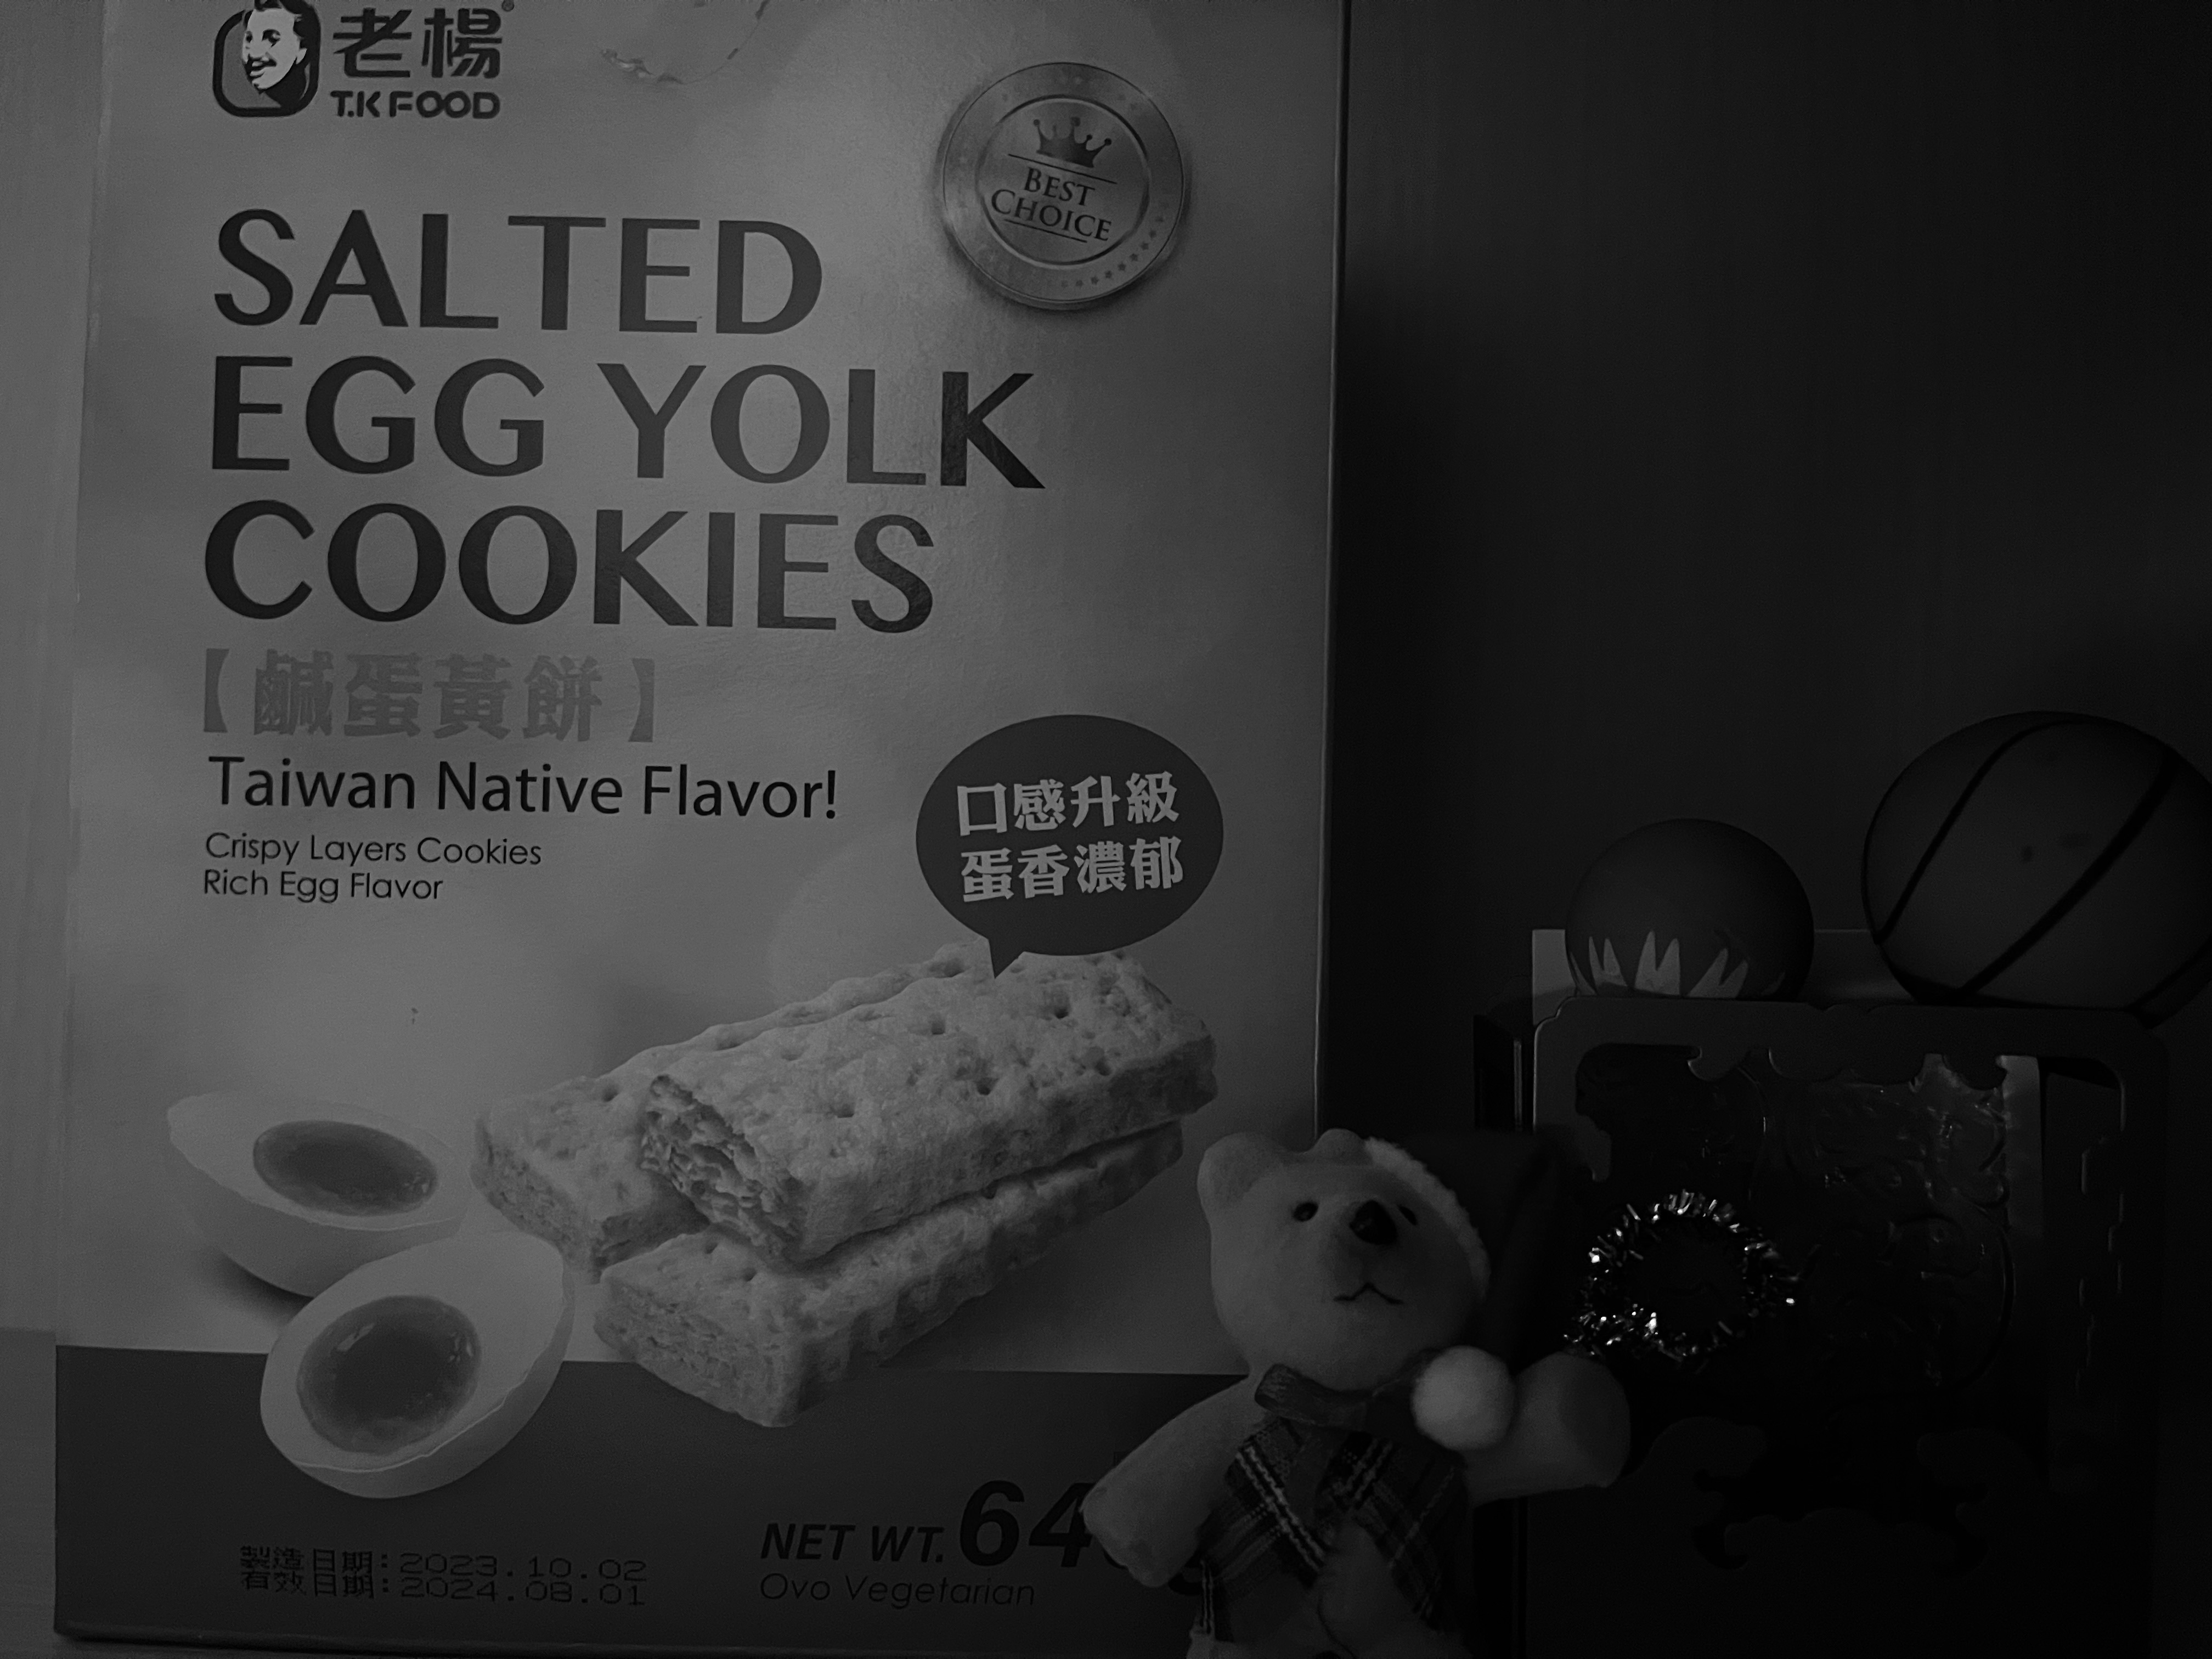
\includegraphics[width=\linewidth]{dark-gray.png}
    \caption{處理前：灰階原圖}
  \end{subfigure}
  \hfill
  \begin{subfigure}[t]{0.48\textwidth}
    \centering
    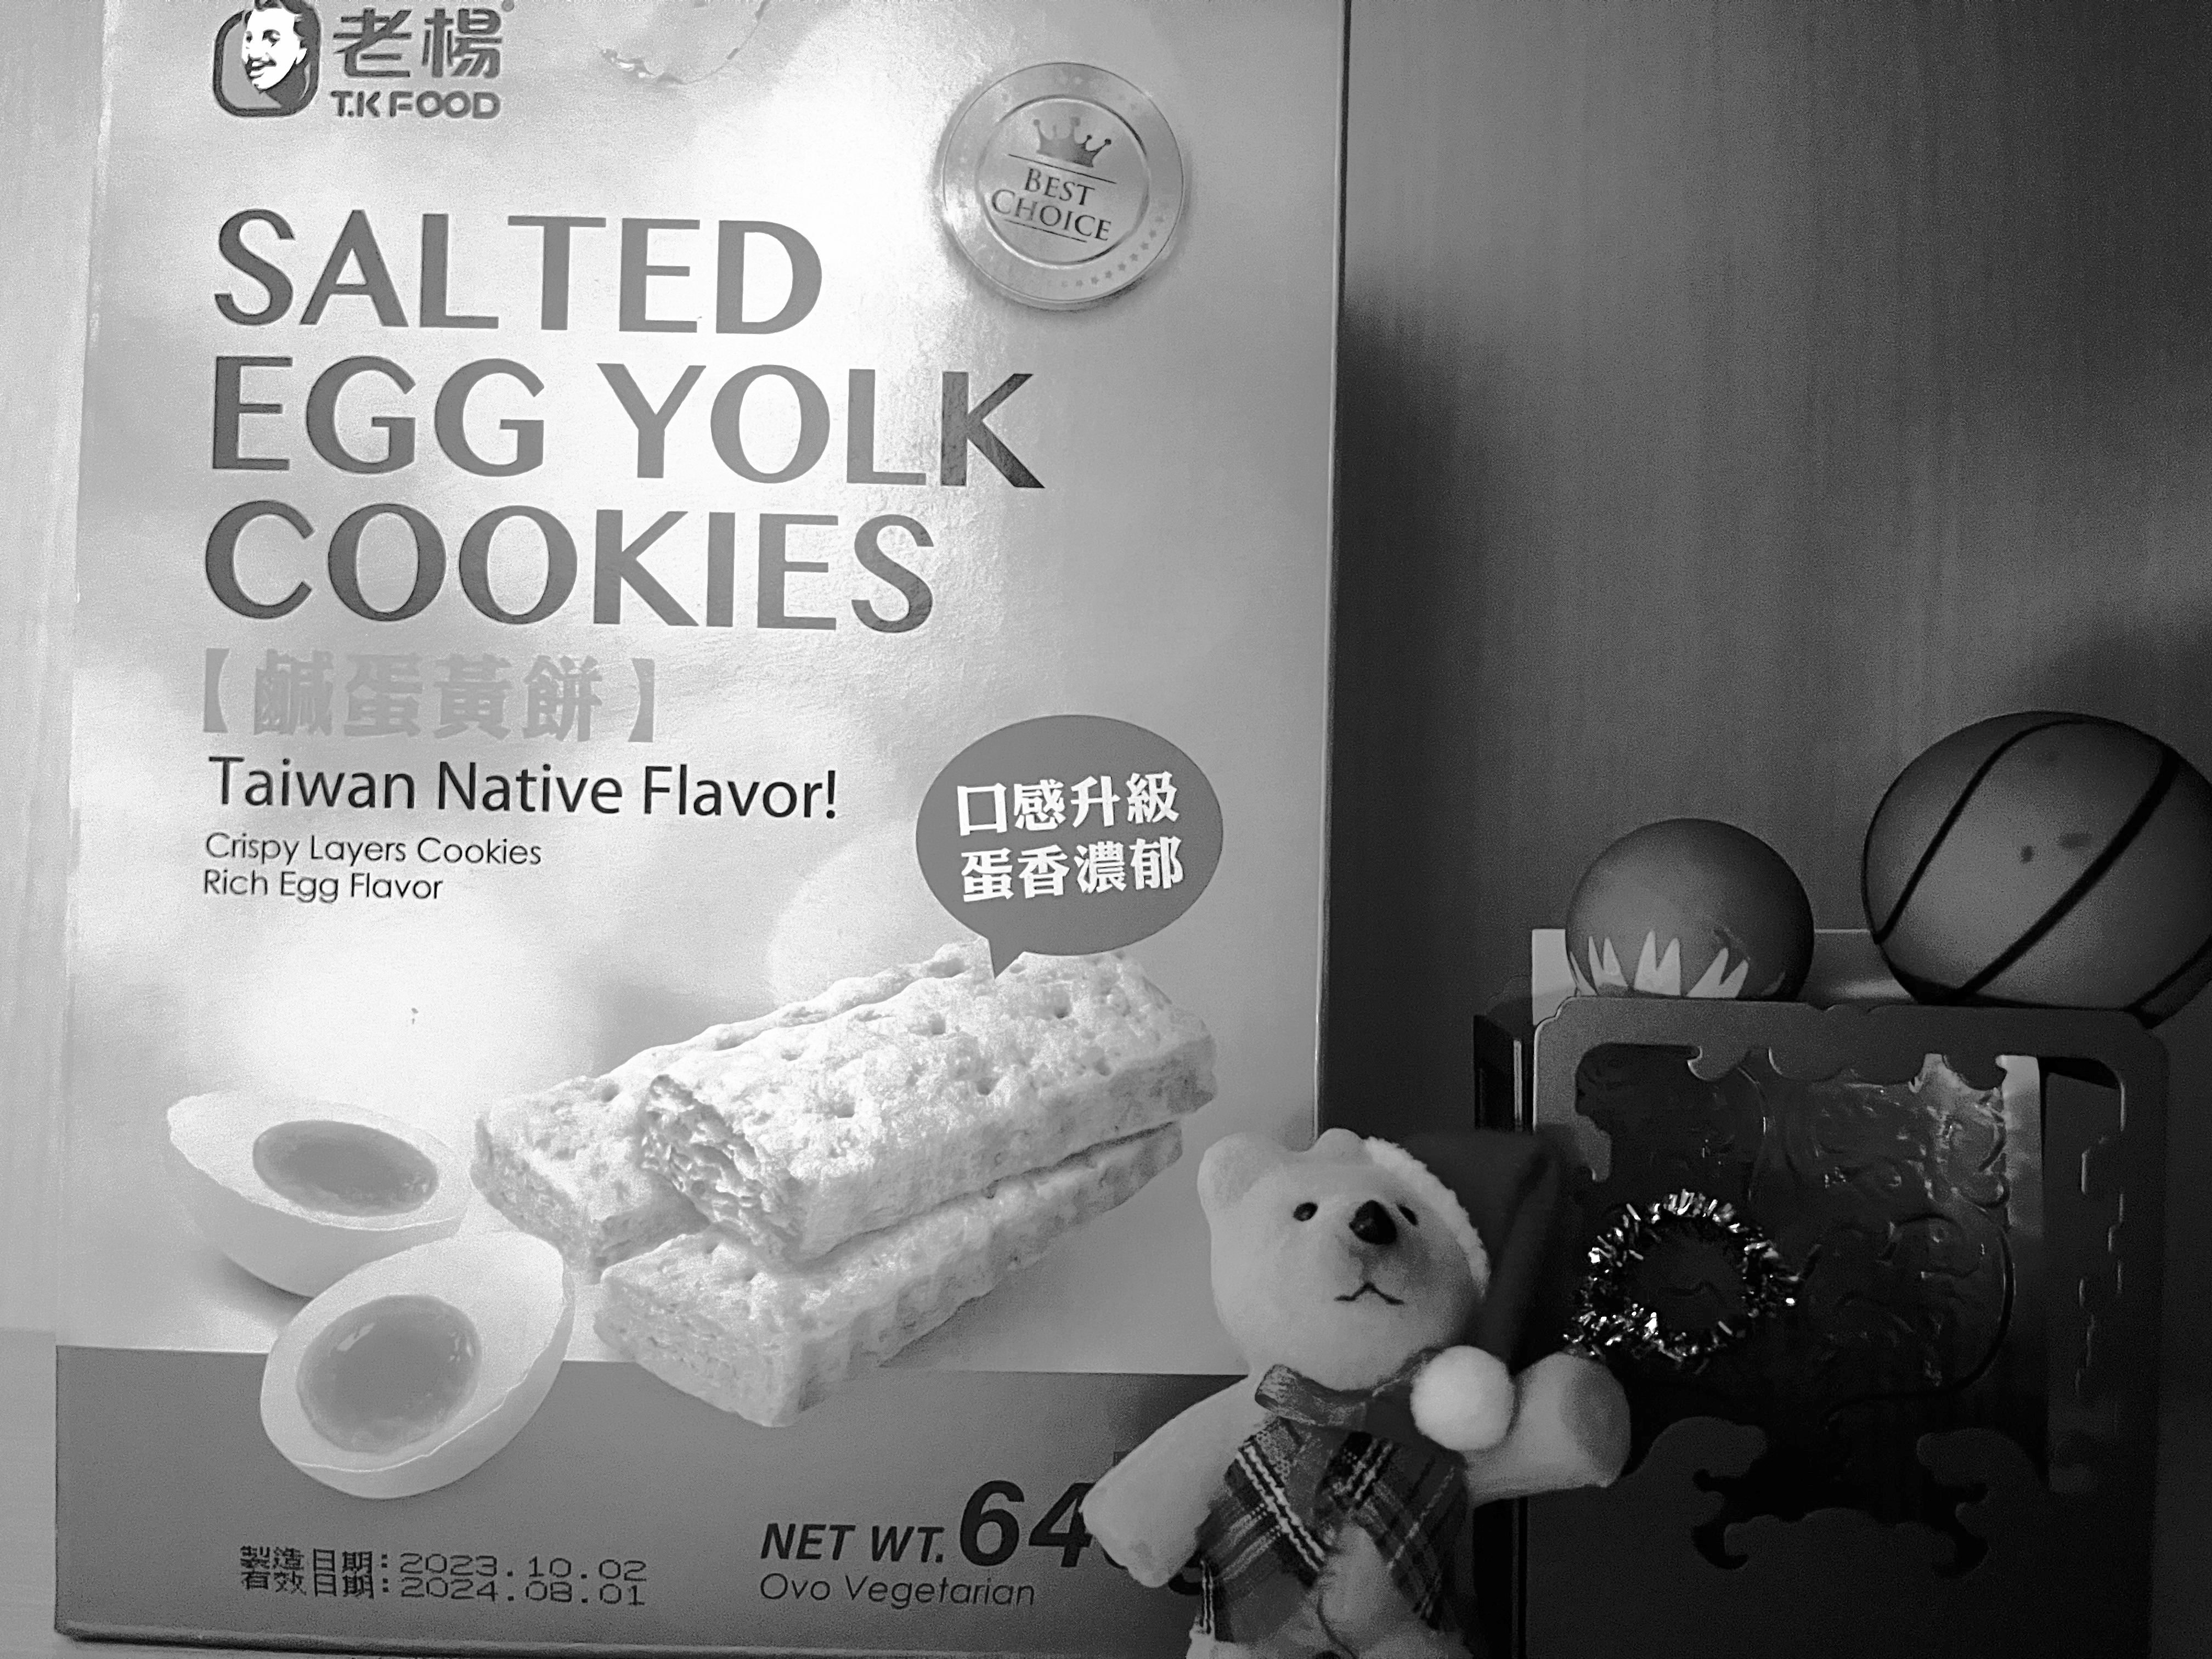
\includegraphics[width=\linewidth]{equalized.png}
    \caption{處理後：直方圖等化}
  \end{subfigure}
  \caption{指定圖片 \texttt{dark.jpg} 的直方圖等化前後比較。}
  \label{fig:histogram-comparison}
\end{figure}

另一方面，餅乾盒左上方與餅乾表面的亮部也變得明亮，
包裝與背景的顆粒感更明顯。
所以本次結果雖有助於辨認暗部物品，並不代表亮部、雜訊與觀看感受都同時改善。
直方圖等化沒有額外執行降噪，也不會辨識哪個區域是觀看者最關心的主體。

\subsection{直方圖與強度映射分析}

圖~\ref{fig:histogram-distributions} 顯示，原圖像素主要集中在低灰階區域，
尤其約 $0$ 至 $120$ 的範圍。
雖然仍有少量高灰階像素，但僅看最小值與最大值無法反映大部分像素偏暗的情況。
等化後，像素分布延伸至較廣的灰階區間，與處理後較明亮、層次差異較大的觀察一致。

\begin{figure}[H]
  \centering
  \begin{subfigure}[t]{0.48\textwidth}
    \centering
    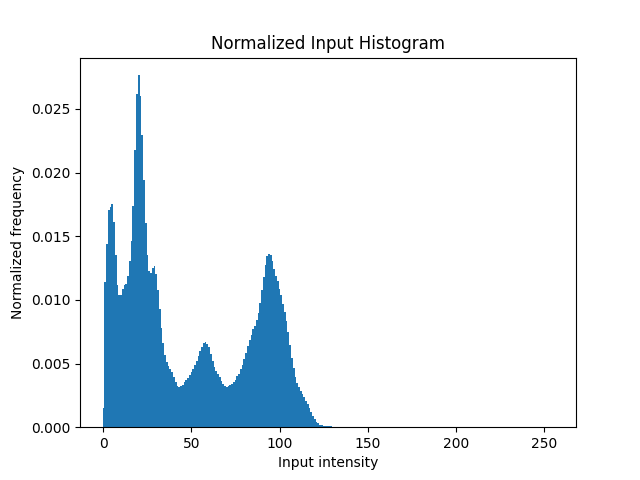
\includegraphics[width=\linewidth]{histogram-input.png}
    \caption{輸入正規化直方圖}
  \end{subfigure}
  \hfill
  \begin{subfigure}[t]{0.48\textwidth}
    \centering
    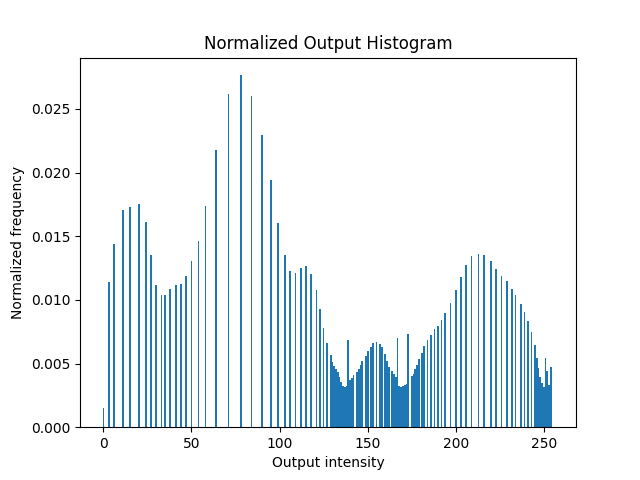
\includegraphics[width=\linewidth]{histogram-output.png}
    \caption{輸出正規化直方圖}
  \end{subfigure}
  \caption{直方圖等化前後的像素灰階比例分布。}
  \label{fig:histogram-distributions}
\end{figure}

輸出直方圖沒有完全平坦，且部分灰階之間存在空隙。
這是離散影像中可能出現的現象：同一個輸入灰階的像素全部映射到同一個輸出值，
無法任意拆分到不同灰階；有限灰階數與取整也會造成跳躍或合併。
因此，不能只以「是否形成水平直線」判斷等化是否正確。

圖~\ref{fig:histogram-mapping} 的映射曲線在像素較集中的灰階區間上升較快，
將這些輸入灰階對應到較廣的輸出範圍；
在像素稀少的高灰階區間，曲線則接近平坦。
這與 CDF 的定義相符，且整條曲線維持單調不減。

\begin{figure}[H]
  \centering
  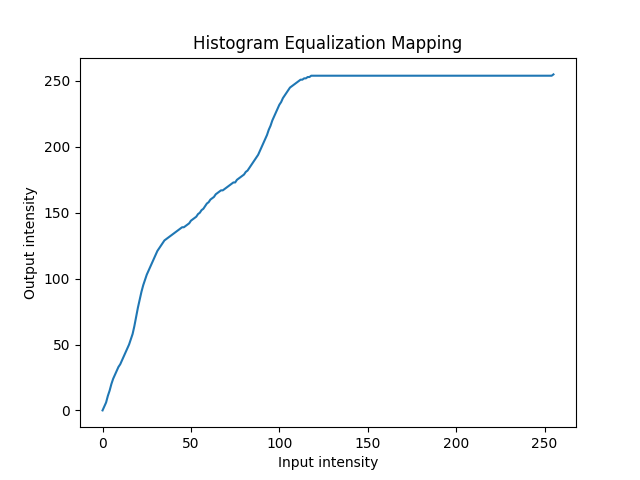
\includegraphics[width=0.72\textwidth]{histogram-mapping.png}
  \caption{輸入灰階至輸出灰階的 CDF 映射。}
  \label{fig:histogram-mapping}
\end{figure}

\subsection{實測數據與結果檢查}

表~\ref{tab:histogram-statistics} 的數值由儲存的完整尺寸 PNG 直接計算。
平均灰階用於描述整體亮度；標準差用於描述像素灰階的整體分散程度，定義為
\begin{equation}
  \sigma(J)=\sqrt{\frac{1}{HW}
    \sum_{y=0}^{H-1}\sum_{x=0}^{W-1}
    \left(J(x,y)-\mu(J)\right)^2}.
  \label{eq:histogram-standard-deviation}
\end{equation}

\begin{table}[H]
  \centering
  \caption{指定圖片的直方圖等化前後統計。}
  \label{tab:histogram-statistics}
  \begin{tabular}{@{}lcc@{}}
    \toprule
    指標 & 處理前 & 處理後 \\
    \midrule
    尺寸（寬 $\times$ 高） & $4032\times3024$ & $4032\times3024$ \\
    資料型態 & \texttt{uint8} & \texttt{uint8} \\
    最小／最大灰階 & $0/255$ & $0/255$ \\
    平均灰階 & $48.68$ & $128.53$ \\
    灰階標準差 & $35.90$ & $73.18$ \\
    正規化直方圖總和 & $1.0$ & $1.0$ \\
    \bottomrule
  \end{tabular}
\end{table}

平均灰階提高，符合原圖偏暗、處理後整體變亮的觀察；
標準差增加，表示灰階在整張圖中的分散程度提高。
兩張圖雖然都具有 $0$ 與 $255$ 的極值，主要灰階分布卻有明顯差異，
因此不能只用輸出是否涵蓋完整灰階範圍來評估效果。
此外，標準差較大不能單獨證明局部細節或主觀品質較好，仍須配合前後圖片分析。

結果檢查包含：確認輸出尺寸與資料型態、核對兩張正規化直方圖總和皆為 $1$，
以及檢查映射是否單調不減。
另外，依原圖重新建立本程式的 CDF 映射後，逐像素對照 \texttt{equalized.png}，
確認儲存結果與式~\eqref{eq:histogram-mapping} 的實作一致。
這些檢查支持程式與輸出的一致性，並不取代影像品質的視覺討論。

\subsection{與 Gamma 轉換的比較及限制}

Gamma 轉換依預先選定的參數改變像素強度，
直方圖等化則依每張影像的灰階比例建立不同的映射。
本次偏暗影像在等化後，文字、餅乾紋理與玩偶輪廓更容易觀看，
但部分亮部也變得很亮，顆粒感較明顯。
兩種方法都屬於全域逐像素強度轉換，
不會根據物體或區域分別設定觀看目標，也無法恢復原圖中已經消失的資訊。
因此，評估時應同時考慮亮度、灰階分布、細節可見度與副作用，不能只以整體變亮判定成功。

\medskip
\noindent\textbf{實作者：}待填。\quad
\textbf{審查者：}待填。\\
\textbf{審查意見：}待實際檢查後填寫。

\clearpage
\section{空間濾波：牙齒與頭骨影像比較}
\label{sec:medical-comparison}

\subsection{實驗目的與處理流程}

此題以 \texttt{pxhere-mouth.jpeg} 的牙齒與下顎影像，
以及 \texttt{wellcome-skull.png} 的頭骨影像測試空間濾波增強。
本節依組員整理的比較觀察，分別討論 Laplacian 與 Sobel 梯度、
Laplacian 與 Mask，以及原圖、直接銳化與 Mask 銳化三組差異，
並以實際輸出圖說明細節增強與細碎反應之間的取捨。

實驗在 \texttt{hw1} 資料夾執行下列指令。
程式先檢查指定的 $3\times3$ 卷積案例，再依序處理兩張圖片，
結果分別儲存於 \texttt{results/medical/mouth} 與
\texttt{results/medical/skull}。

\begin{lstlisting}[language={},caption={醫學影像增強實驗的執行指令}]
python medical_experiments.py
\end{lstlisting}

表~\ref{tab:medical-stages} 列出下列比較所使用的處理階段。
兩張影像採用相同設定：Laplacian 為中央係數 $8$、周圍八個係數 $-1$ 的
$3\times3$ 核心；Sobel 使用水平與垂直兩個 $3\times3$ 核心，
再計算梯度大小；Box filter 的半徑為 $2$，即 $5\times5$，各係數為 $1/25$。

\begin{table}[H]
  \centering
  \caption{醫學影像比較所用的輸出階段。}
  \label{tab:medical-stages}
  \begin{tabularx}{\textwidth}{@{}lX@{}}
    \toprule
    輸出檔名 & 處理內容 \\
    \midrule
    \texttt{0-gray.png} & 灰階原圖 $I$。 \\
    \texttt{1-laplacian.png} & Laplacian 細節影像 $L$。 \\
    \texttt{2-gradient.png} & Sobel 梯度大小影像。 \\
    \texttt{3-smoothed-gradient.png} & 經 $5\times5$ Box filter 平滑的梯度影像 $S$。 \\
    \texttt{4-sharpened.png} & 將 $L$ 加回原圖，得到直接銳化結果。 \\
    \texttt{5-mask.png} & 將 $L$ 與 $S$ 正規化後逐像素相乘，得到 Mask。 \\
    \texttt{6-denoised\_sharpened.png} & 將 Mask 加回原圖，得到調整增強量後的結果。 \\
    \bottomrule
  \end{tabularx}
\end{table}

Laplacian 與梯度影像依程式設定截斷至 $[0,255]$，並轉為八位元影像；
因此，下列觀察對應的是程式輸出的可視化結果，Laplacian 的負反應未保留在輸出 PNG 中。
Mask 的乘法在正規化後進行，可視為使用平滑梯度調整各位置的 Laplacian 增強量。
梯度較弱的位置通常加入較少細節，梯度較強的位置則保留較多反應。
為觀察濾波與銳化本身的效果，下列三組比較皆使用最後 Gamma 提亮之前的影像。

\subsection{六個運算函式的 TODO 實作與說明}
\label{sec:medical-implementation}

以下六個函式取自 \texttt{spatial\_operations.py}，省略原始註解與空行，
保留實際運算、資料型態轉換及回傳步驟。
輸入影像皆為二維灰階影像；除卷積測試使用浮點矩陣外，
本實驗傳入各濾波與影像乘加函式的像素值均位於 $[0,255]$。
除以 $255$ 是依固定灰階範圍縮放，並非依每張圖片的最大值與最小值重新拉伸。
運算前轉為浮點數可保留負值與小數，避免直接以 \texttt{uint8} 做乘加時發生溢位。

\subsubsection{\textnormal{\texttt{convolution}}：補零與二維卷積}

\noindent\begin{minipage}{\linewidth}
\begin{lstlisting}[caption={自行實作補零與兩層迴圈卷積},label={lst:medical-convolution}]
def convolution(input_image, kernel):
    output_image = input_image.copy()
    height, width = input_image.shape
    size = kernel.shape[0]
    if kernel.shape != (size, size) or size % 2 == 0:
        raise ValueError('The kernel must be a square with odd side length.')
    radius = size // 2
    padded_image = np.pad(input_image.astype(float), radius, mode='constant')
    output_image = np.zeros((height, width), dtype=float)
    flipped_kernel = kernel[::-1, ::-1]
    for y in range(height):
        for x in range(width):
            region = padded_image[y:y + size, x:x + size]
            output_image[y, x] = np.sum(region * flipped_kernel)
    return output_image
\end{lstlisting}
\end{minipage}\par

程式~\ref{lst:medical-convolution} 先檢查核心是否為奇數邊長的方形矩陣，
使中心位置與半徑 $r=\lfloor\texttt{size}/2\rfloor$ 能明確定義。
\texttt{np.pad} 在上、下、左、右各補 $r$ 個零，
因此原圖邊界也能取出完整視窗，輸出仍維持原本的高與寬。
\texttt{kernel[::-1, ::-1]} 將核心的列與欄順序反轉，相當於旋轉 $180$ 度，
符合本題採用的數學卷積定義。
兩層 \texttt{for} 分別遍歷列 $y$ 與欄 $x$，
切出局部區塊後，以 NumPy 做逐項乘法與加總，未呼叫第三方卷積 API。
若核心邊長為 $2r+1$，實際計算式為
\begin{equation}
  O[y,x]=\sum_{i=0}^{2r}\sum_{j=0}^{2r}
  I_{\mathrm{pad}}[y+i,x+j]\,K[2r-i,2r-j].
  \label{eq:medical-convolution}
\end{equation}
輸出採浮點數且未截斷，可保留卷積結果的小數與正負號；
是否縮放、截斷或轉成八位元影像，交由呼叫它的濾波函式處理。

\subsubsection{\textnormal{\texttt{box\_filter}}：局部平均與實際 Box 核心}

\noindent\begin{minipage}{\linewidth}
\begin{lstlisting}[caption={依半徑建立正規化 Box 核心並平滑影像},label={lst:medical-box}]
def box_filter(input_image, radius):
    output_image = input_image.copy().astype(float)
    output_image /= 255
    size = 2 * radius + 1
    kernel = np.ones((size, size), dtype=float) / (size * size)
    output_image = convolution(output_image, kernel)
    output_image *= 255
    output_image = output_image.astype(np.uint8)
    return output_image
\end{lstlisting}
\end{minipage}\par

程式~\ref{lst:medical-box} 先將灰階值縮放到 $[0,1]$，
再建立邊長為 $2r+1$ 的全一矩陣，並除以元素數量 $(2r+1)^2$，
使所有係數總和為 $1$，卷積結果即為鄰域的平均值。
本實驗對梯度影像使用半徑 $r=2$，實際核心為
\begin{equation}
  K_{\mathrm{Box}}=\frac{1}{25}
  \begin{bmatrix}
    1&1&1&1&1\\
    1&1&1&1&1\\
    1&1&1&1&1\\
    1&1&1&1&1\\
    1&1&1&1&1
  \end{bmatrix}.
  \label{eq:medical-box-kernel}
\end{equation}
平滑梯度影像可將局部梯度反應取平均，作為後續 Mask 的權重。
卷積後乘回 $255$，並轉為 \texttt{uint8}；非負小數部分會在轉型時截去。
因為核心係數非負且總和為 $1$，對本實驗的輸入可維持灰階範圍。
但邊界採補零，常數影像的邊緣也可能因納入外側零值而變暗。

\subsubsection{\textnormal{\texttt{laplacian\_filter}}：二階差分與實際 Laplacian 核心}

\noindent\begin{minipage}{\linewidth}
\begin{lstlisting}[caption={使用中心為正的八鄰居 Laplacian 核心},label={lst:medical-laplacian}]
def laplacian_filter(input_image):
    output_image = input_image.copy().astype(float)
    output_image /= 255
    kernel = np.array([[-1, -1, -1],
                       [-1,  8, -1],
                       [-1, -1, -1]], dtype=float)
    output_image = convolution(output_image, kernel)
    output_image *= 255
    output_image[output_image > 255] = 255
    output_image[output_image < 0] = 0
    output_image = output_image.astype(np.uint8)
    return output_image
\end{lstlisting}
\end{minipage}\par

程式~\ref{lst:medical-laplacian} 選擇中央係數為正的八鄰居核心，實際矩陣為
\begin{equation}
  K_{\mathrm{L}}=
  \begin{bmatrix}
    -1&-1&-1\\
    -1& 8&-1\\
    -1&-1&-1
  \end{bmatrix}.
  \label{eq:medical-laplacian-kernel}
\end{equation}
其係數總和為 $0$，運算相當於「中心值的八倍減去八個鄰居的總和」，
因此在不受補零邊界影響的常數區域反應為零，亮度快速變化處則有較大反應。
以連續微分的符號來看，此中心為正的形式對應負的 Laplacian，
故可依本題流程將其反應加回原圖以增強細節。
本實作在乘回 $255$ 後，將大於 $255$ 的值設為 $255$、負值設為 $0$，
再轉為 \texttt{uint8}。
因此後續銳化使用的是經截斷的非負細節影像，並未保留完整的帶正負號二階差分；
截斷會移除負反應與過大反應的幅值差異，也可能使加回後的亮部飽和。

\subsubsection{\textnormal{\texttt{sobel\_filter}}：方向梯度、大小與實際 Sobel 核心}

\noindent\begin{minipage}{\linewidth}
\begin{lstlisting}[caption={以兩個 Sobel 核心計算梯度大小},label={lst:medical-sobel}]
def sobel_filter(input_image):
    output_image = input_image.copy().astype(float)
    output_image /= 255
    kernel_x = np.array([[-1, 0, 1],
                         [-2, 0, 2],
                         [-1, 0, 1]], dtype=float)
    kernel_y = np.array([[-1, -2, -1],
                         [ 0,  0,  0],
                         [ 1,  2,  1]], dtype=float)
    gx = convolution(output_image, kernel_x)
    gy = convolution(output_image, kernel_y)
    output_image = np.sqrt(gx ** 2 + gy ** 2)
    output_image *= 255
    output_image[output_image > 255] = 255
    output_image = output_image.astype(np.uint8)
    return output_image
\end{lstlisting}
\end{minipage}\par

程式~\ref{lst:medical-sobel} 使用下列兩個核心，分別取得左右方向 $x$ 與上下方向 $y$ 的亮度變化：
\begin{equation}
  K_x=
  \begin{bmatrix}
    -1&0&1\\
    -2&0&2\\
    -1&0&1
  \end{bmatrix},
  \qquad
  K_y=
  \begin{bmatrix}
    -1&-2&-1\\
     0& 0& 0\\
     1& 2& 1
  \end{bmatrix}.
  \label{eq:medical-sobel-kernels}
\end{equation}
令正規化原圖為 $I_n=I/255$，先透過自行實作的卷積得到
$g_x=I_n*K_x$、$g_y=I_n*K_y$，再依
\begin{equation}
  G(x,y)=\sqrt{g_x(x,y)^2+g_y(x,y)^2}
  \label{eq:medical-gradient-magnitude}
\end{equation}
合成梯度大小。\texttt{** 2} 表示逐元素平方，\texttt{np.sqrt} 為逐元素開根號，
因此同時考慮兩方向的變化，且結果非負。
由於卷積會旋轉核心，上列反對稱 Sobel 核心相較於不旋轉的互相關運算，
方向反應的符號會反轉，但平方後的梯度大小不受此符號差異影響。
程式沒有另外將 Sobel 係數除以 $8$，而是直接將梯度大小乘回 $255$，
把超過 $255$ 的值截斷後轉為 \texttt{uint8}。
因此輸出強度同時受核心倍率與飽和截斷影響，不能直接當作未截斷的梯度數值。

\subsubsection{\textnormal{\texttt{image\_product}}：正規化後逐像素相乘}

\noindent\begin{minipage}{\linewidth}
\begin{lstlisting}[caption={將平滑梯度作為 Laplacian 細節的逐像素權重},label={lst:medical-product}]
def image_product(input_image_a, input_image_b):
    input_image_a = input_image_a.astype(float)
    input_image_b = input_image_b.astype(float)
    input_image_a /= 255
    input_image_b /= 255
    output_image = input_image_a.copy()
    output_image = input_image_a * input_image_b
    output_image *= 255
    output_image = output_image.astype(np.uint8)
    return output_image
\end{lstlisting}
\end{minipage}\par

程式~\ref{lst:medical-product} 先將兩張同尺寸影像轉為浮點數並除以 $255$，
再以 \texttt{*} 對相同位置的像素相乘，最後乘回 $255$ 並轉為 \texttt{uint8}。
這是逐元素乘法，不是矩陣乘法。
對本實驗的 Laplacian 影像 $L$ 與平滑梯度影像 $S$，轉型前的 Mask 計算為
\begin{equation}
  M_{\mathrm{float}}(x,y)
  =255\left(\frac{L(x,y)}{255}\right)
       \left(\frac{S(x,y)}{255}\right)
  =\frac{L(x,y)S(x,y)}{255}.
  \label{eq:medical-mask}
\end{equation}
由於 $S/255$ 位於 $[0,1]$，它可作為每個位置的增強權重：
梯度較弱處減少加入的細節，較強處保留較多 Laplacian 反應。
例如 $L=128$、$S=64$ 時，乘回灰階範圍後約為 $32.13$，轉型後為 $32$。
兩個非負且不超過 $1$ 的正規化值相乘仍位於 $[0,1]$，因此本流程不需額外截斷。

\subsubsection{\textnormal{\texttt{image\_sum}}：逐像素相加與飽和截斷}

\noindent\begin{minipage}{\linewidth}
\begin{lstlisting}[caption={將細節影像加回原圖並限制最大灰階},label={lst:medical-sum}]
def image_sum(input_image_a, input_image_b):
    input_image_a = input_image_a.astype(float)
    input_image_b = input_image_b.astype(float)
    input_image_a /= 255
    input_image_b /= 255
    output_image = input_image_a.copy()
    output_image = input_image_a + input_image_b
    output_image *= 255
    output_image[output_image > 255] = 255
    output_image = output_image.astype(np.uint8)
    return output_image
\end{lstlisting}
\end{minipage}\par

程式~\ref{lst:medical-sum} 先轉為浮點數並正規化，再以 \texttt{+} 做逐像素相加。
兩個正規化像素相加後可能大於 $1$，因此乘回 $255$ 後須將超過 $255$ 的值截斷，
避免轉為八位元整數時溢位；本實驗兩張輸入皆非負，故沒有負值需要處理。
不考慮浮點捨入與轉型截斷時，此運算等價於 $\min(255,A+B)$，
實際整數結果則依上述浮點計算及 \texttt{uint8} 轉型取得。
本流程以 \texttt{image\_sum} 將原圖分別與 Laplacian 影像及 Mask 影像相加，
產生直接銳化與 Mask 銳化影像。
兩者都採加法，但 Mask 先透過平滑梯度減少部分細節增強量，
因此與直接加入 Laplacian 的結果有所差異；兩者仍可能出現亮部飽和。

\subsection{補零示意與指定卷積測試}
\label{sec:medical-convolution-test}

\subsubsection{指定 3×3 卷積測試與輸出數值}

為檢查程式~\ref{lst:medical-convolution} 的補零、核心旋轉與邊界計算，
\texttt{medical\_experiments.py} 使用作業指定的輸入矩陣與非對稱核心：
\begin{equation}
  I_{\mathrm{test}}=
  \begin{bmatrix}1&2&3\\4&5&6\\7&8&9\end{bmatrix},
  \qquad
  K_{\mathrm{test}}=\frac{1}{7}
  \begin{bmatrix}-1&1&1\\-1&1&1\\1&1&1\end{bmatrix}.
\end{equation}
此時 $r=1$，影像四周各補一個零，得到
\begin{equation}
  I_{\mathrm{pad}}=
  \begin{bmatrix}
    0&0&0&0&0\\
    0&1&2&3&0\\
    0&4&5&6&0\\
    0&7&8&9&0\\
    0&0&0&0&0
  \end{bmatrix}.
\end{equation}
依數學卷積定義旋轉核心後，實測結果為
\begin{equation}
  O_{\mathrm{test}}=\frac{1}{7}
  \begin{bmatrix}-2&3&16\\1&15&33\\8&21&28\end{bmatrix}.
  \label{eq:medical-convolution-test-output}
\end{equation}
儲存在 \texttt{convolution-test.csv} 的結果保留小數點後八位，數值如下：
\begin{equation}
  O_{\mathrm{CSV}}=
  \begin{bmatrix}
    -0.28571429&0.42857143&2.28571429\\
     0.14285714&2.14285714&4.71428571\\
     1.14285714&3.00000000&4.00000000
  \end{bmatrix}.
  \label{eq:medical-convolution-csv}
\end{equation}
此矩陣為式~\ref{eq:medical-convolution-test-output} 的小數表示，
CSV 與精確分數矩陣的最大絕對差約為 $4.29\times10^{-9}$，來自存檔時的小數位數限制。
例如左上角視窗使用旋轉後的核心，得到
$(1-2+4-5)/7=-2/7$，顯示卷積函式保留負值，而非在此階段歸零。
測試程式以 \texttt{np.testing.assert\_allclose} 與預期矩陣比較，
設定絕對容許誤差為 $10^{-12}$，並輸出
\texttt{results/medical/convolution-test.csv} 與圖~\ref{fig:medical-convolution-test}。
此非對稱核心也能區分「有旋轉核心的卷積」與「不旋轉核心的互相關」。

\begin{figure}[H]
  \centering
  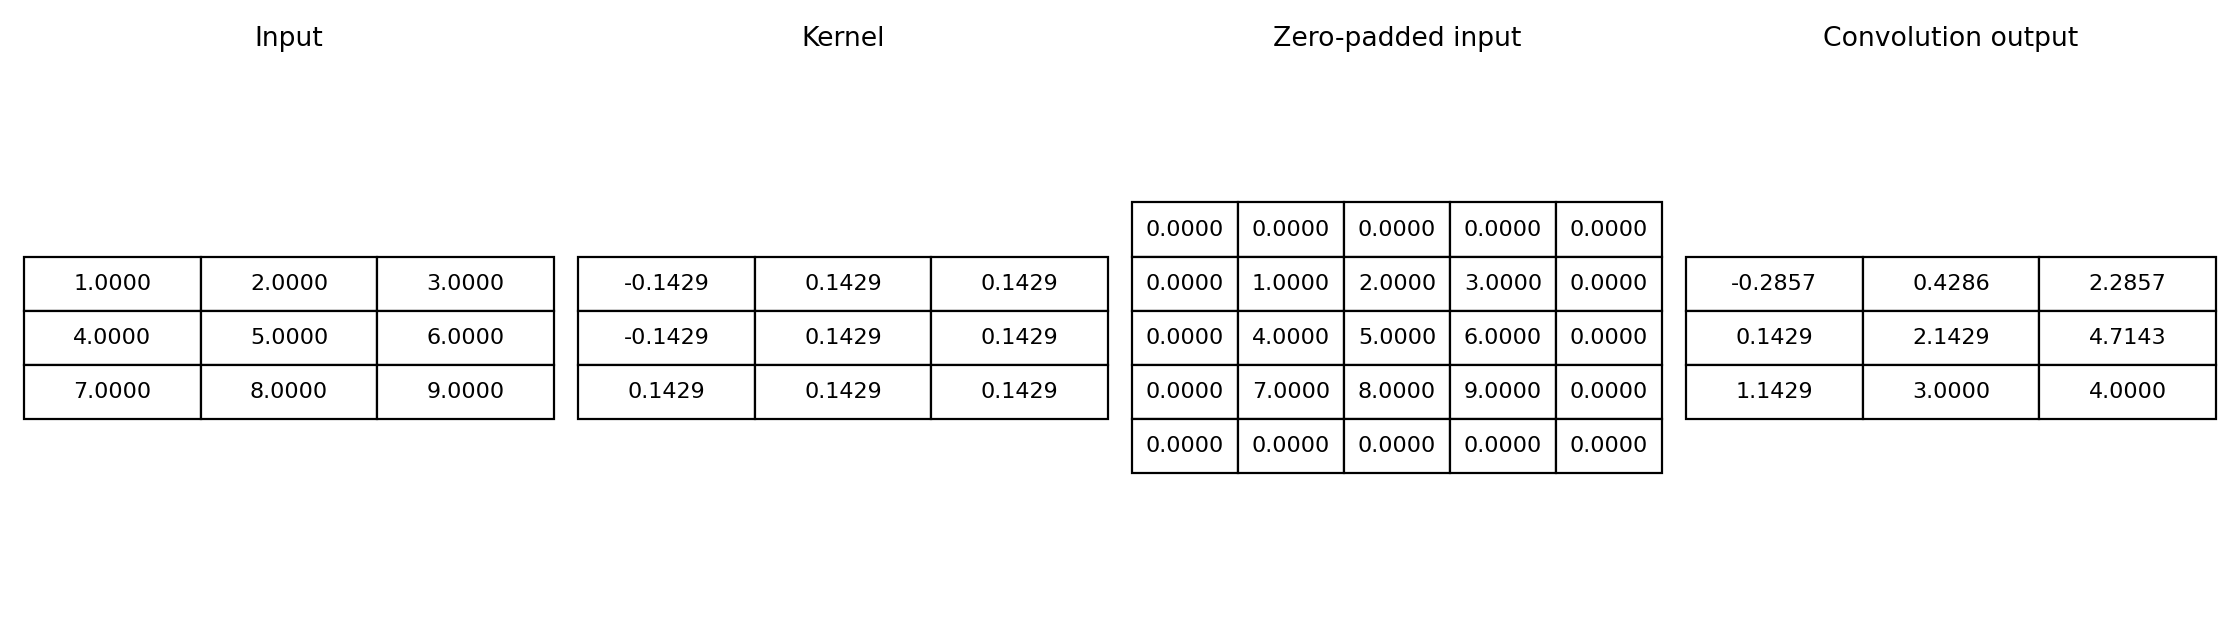
\includegraphics[width=\textwidth]{medical/convolution-test.png}
  \caption{指定卷積測試的輸入、核心、補零矩陣與輸出數值；圖中數值顯示至小數第四位，精確結果如式~\ref{eq:medical-convolution-test-output}。}
  \label{fig:medical-convolution-test}
\end{figure}

實際影像同樣採補零：Laplacian 與 Sobel 的 $3\times3$ 核心每側補 $1$ 個像素，
Box 的 $5\times5$ 核心每側補 $2$ 個像素。
補零影像是運算用的中間陣列，最終濾波輸出的高寬仍與輸入相同。

\subsubsection{實際影像的補零圖片與驗證}
\label{sec:medical-padding-images}

兩組補零素材位於 \texttt{results/medical} 下的 \texttt{mouth} 與 \texttt{skull} 資料夾。
圖~\ref{fig:medical-mouth-padding} 與圖~\ref{fig:medical-skull-padding}
分別展示兩個案例的 \texttt{padded.png}（補零全圖）與
\texttt{padding-detail.png}（左上角放大圖）。
兩組素材皆示範半徑 $r=1$ 的補零，對應 $3\times3$ 核心：
原影像的上、下、左、右各新增一個像素寬的零值邊框，
高寬由 $H\times W$ 變為 $(H+2)\times(W+2)$。
表~\ref{tab:medical-padding-check} 列出直接讀取影像檔案後核對的尺寸與像素結果。

\begin{table}[H]
  \centering
  \caption{實際補零影像的檢查結果；尺寸順序為高 $\times$ 寬，單位為像素。}
  \label{tab:medical-padding-check}
  \begin{tabular}{@{}lccc@{}}
    \toprule
    案例 & 原灰階影像 & 每側補一個零後 & 四側新增像素值 \\
    \midrule
    牙齒與下顎 & $150\times336$ & $152\times338$ & 全為 $0$ \\
    頭骨 & $900\times1100$ & $902\times1102$ & 全為 $0$ \\
    \bottomrule
  \end{tabular}
\end{table}

除尺寸外，也逐像素確認補零圖的內部區域
\texttt{padded[1:-1, 1:-1]} 與原灰階圖完全一致，
且第一列、最後一列、第一欄及最後一欄皆為 $0$。
因此新增的只有零值邊框，影像內部並未因補零而改變。
左上角放大圖中，座標 $0$ 的列與欄所形成的黑色帶即為新增邊框；
影像本身原有的亮色邊緣仍保留在框內。

\begin{figure}[H]
  \centering
  \begin{subfigure}[t]{0.48\textwidth}
    \centering
    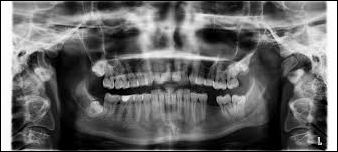
\includegraphics[width=\linewidth,height=0.25\textheight,keepaspectratio]{medical/mouth/padded.png}
    \caption{補零全圖：$152\times338$}
  \end{subfigure}
  \hfill
  \begin{subfigure}[t]{0.48\textwidth}
    \centering
    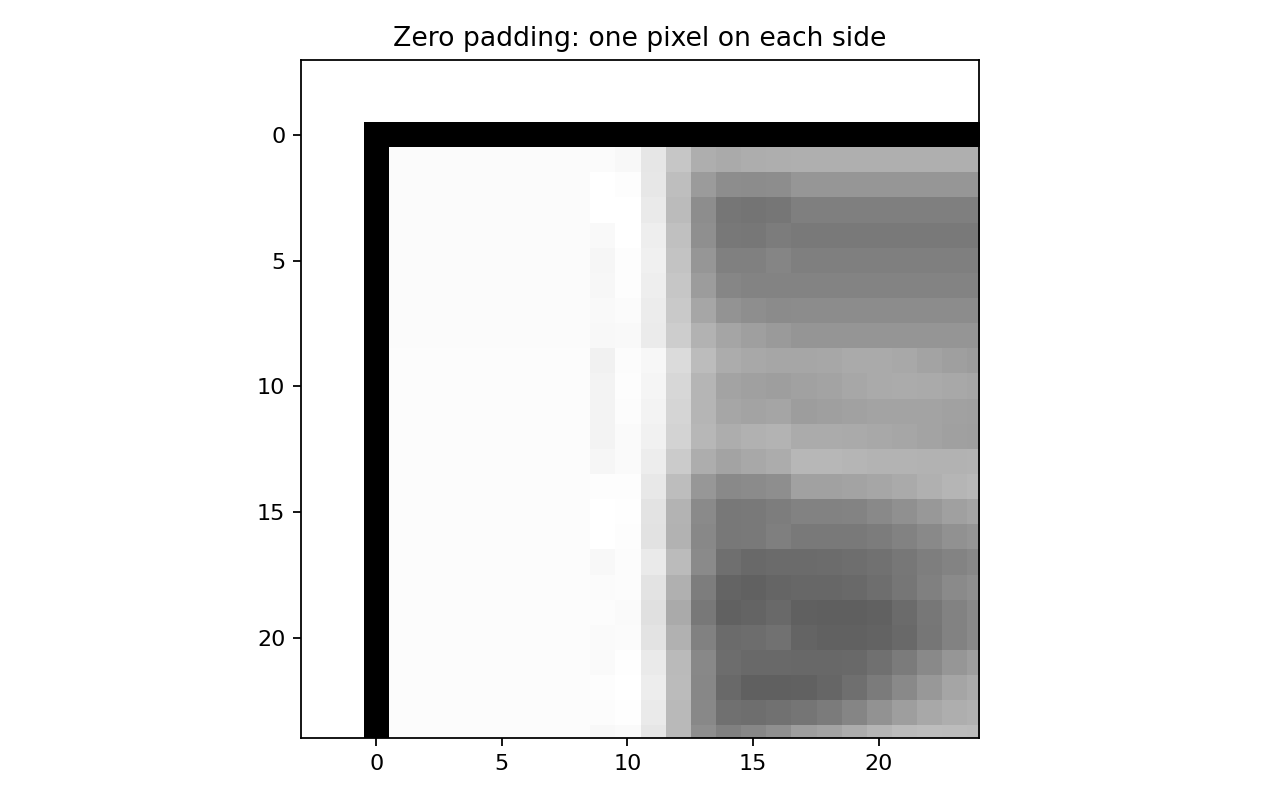
\includegraphics[width=\linewidth,height=0.25\textheight,keepaspectratio]{medical/mouth/padding-detail.png}
    \caption{左上角放大：顯示新增零值邊框}
  \end{subfigure}
  \caption{牙齒與下顎影像每側補一個零值像素後的全圖與局部放大。}
  \label{fig:medical-mouth-padding}
\end{figure}

\begin{figure}[H]
  \centering
  \begin{subfigure}[t]{0.48\textwidth}
    \centering
    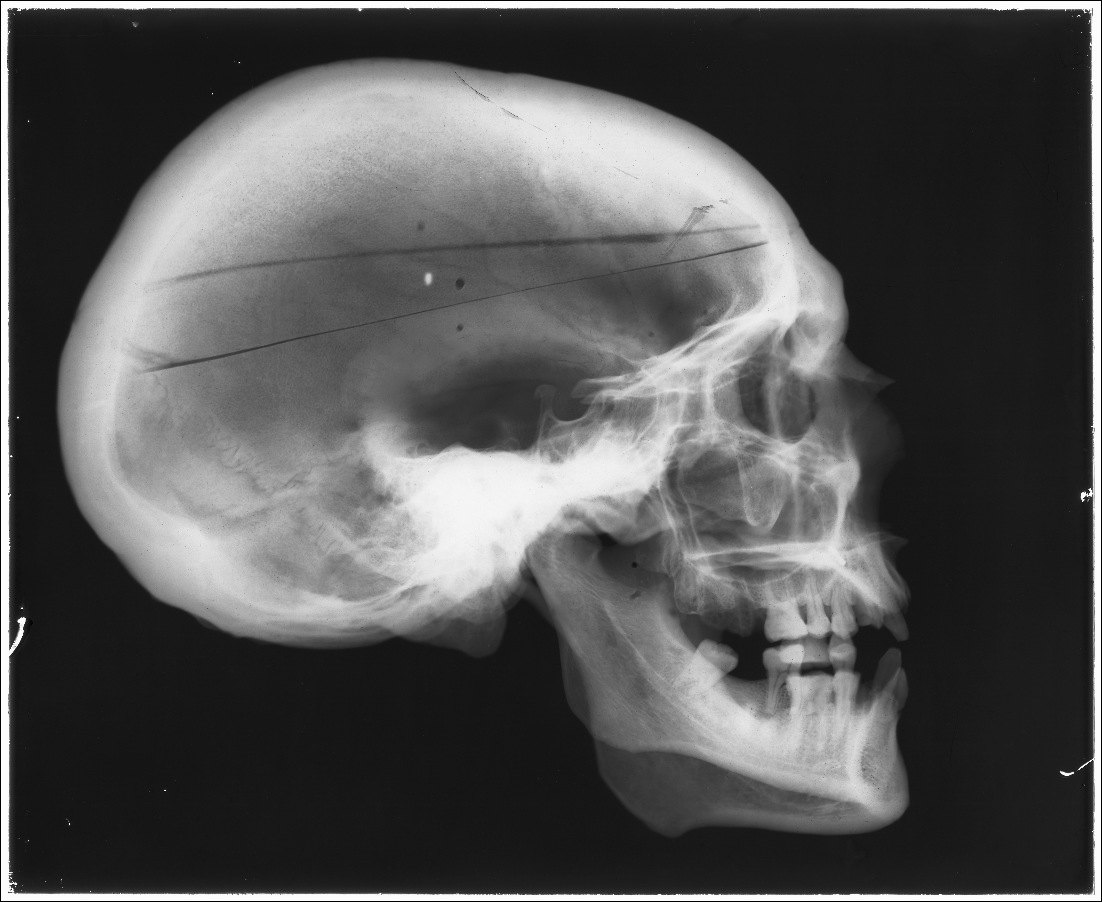
\includegraphics[width=\linewidth,height=0.25\textheight,keepaspectratio]{medical/skull/padded.png}
    \caption{補零全圖：$902\times1102$}
  \end{subfigure}
  \hfill
  \begin{subfigure}[t]{0.48\textwidth}
    \centering
    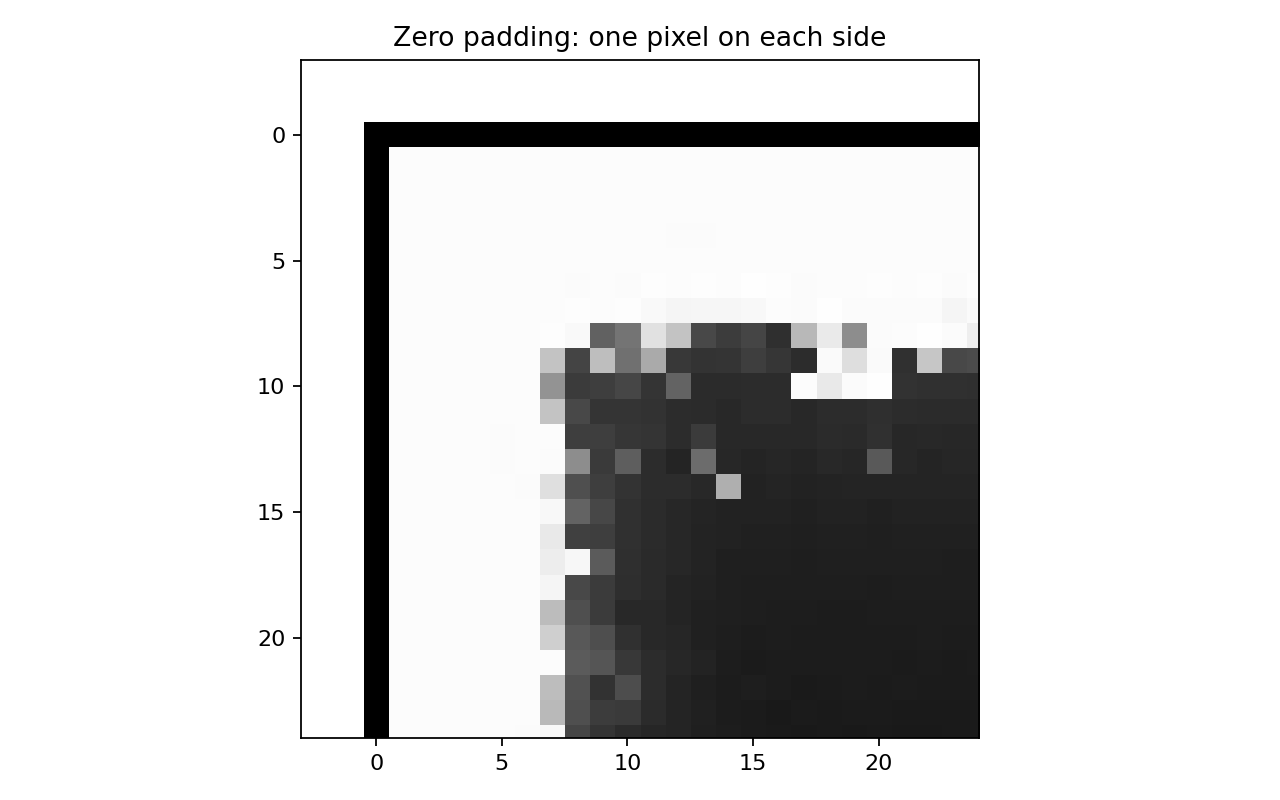
\includegraphics[width=\linewidth,height=0.25\textheight,keepaspectratio]{medical/skull/padding-detail.png}
    \caption{左上角放大：顯示新增零值邊框}
  \end{subfigure}
  \caption{頭骨影像每側補一個零值像素後的全圖與局部放大。}
  \label{fig:medical-skull-padding}
\end{figure}

若使用半徑 $r=2$ 的 $5\times5$ Box 核心，依同一規則每側補兩個零值像素，
運算陣列的尺寸為 $(H+4)\times(W+4)$。
無論使用哪一個半徑，卷積函式都只輸出原影像的 $H\times W$ 個位置，
因此不能將補零後的中間陣列尺寸誤認為濾波結果尺寸。
補零也假設影像外側亮度為零，靠近邊界的濾波反應可能因此不同於影像內部。

\subsection{牙齒與下顎影像}

\subsubsection{Laplacian 與 Gradient 比較}

如圖~\ref{fig:mouth-laplacian-gradient}，Laplacian 呈現較細碎的線條與點狀紋理，
牙齒及下顎周圍的反應較零散。
Gradient 中的牙齒邊界與下顎輪廓則較明亮、粗且連續，主要結構更容易辨認。
這與兩者的運算特性一致：Laplacian 使用二階差分，對局部快速變化較敏感；
Sobel 梯度大小則整合兩個方向的一階變化，使主要邊界較突出。
圖像亮暗也受到核心係數、幅值與截斷方式影響，不能只以線條較亮判斷方法優劣。

\begin{figure}[H]
  \centering
  \begin{subfigure}[t]{0.48\textwidth}
    \centering
    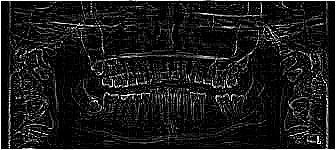
\includegraphics[width=\linewidth]{medical/mouth/1-laplacian.png}
    \caption{Laplacian}
  \end{subfigure}
  \hfill
  \begin{subfigure}[t]{0.48\textwidth}
    \centering
    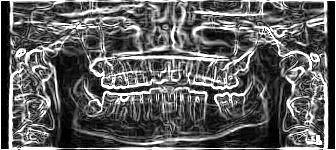
\includegraphics[width=\linewidth]{medical/mouth/2-gradient.png}
    \caption{Sobel Gradient}
  \end{subfigure}
  \caption{牙齒與下顎影像的 Laplacian 與梯度大小比較。}
  \label{fig:mouth-laplacian-gradient}
\end{figure}

\subsubsection{Laplacian 與 Mask 比較}

如圖~\ref{fig:mouth-laplacian-mask}，相較於 Laplacian，Mask 整體較暗，
牙齒與下顎周圍的部分細碎反應減弱，主要輪廓仍有保留。
原因是平滑梯度作為逐像素權重，使梯度較弱處的 Laplacian 反應受到抑制。
Mask 變暗是乘法調整增強量的結果；同時也可能削弱有用的微小紋理，
所以需要連同主要輪廓與細節的保留程度一起評估。

\begin{figure}[H]
  \centering
  \begin{subfigure}[t]{0.48\textwidth}
    \centering
    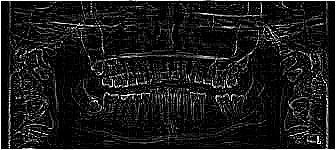
\includegraphics[width=\linewidth]{medical/mouth/1-laplacian.png}
    \caption{Laplacian}
  \end{subfigure}
  \hfill
  \begin{subfigure}[t]{0.48\textwidth}
    \centering
    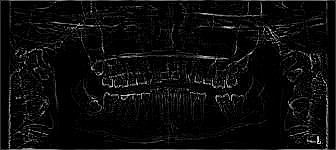
\includegraphics[width=\linewidth]{medical/mouth/5-mask.png}
    \caption{Mask}
  \end{subfigure}
  \caption{牙齒與下顎影像的 Laplacian 與 Mask 比較。}
  \label{fig:mouth-laplacian-mask}
\end{figure}

\subsubsection{原圖、Sharpened 與 Denoised Sharpened 比較}

如圖~\ref{fig:mouth-sharpening}，相較於原圖，直接銳化的 Sharpened 在牙齒周圍
及下顎輪廓的邊緣更明顯，但也增加了細碎點狀反應、顆粒感與過強的亮線。
將 Mask 加回原圖的 Denoised Sharpened，則減弱了這些額外反應，
仍保留主要牙齒與下顎輪廓，整體較接近原圖。
不過，牙齒內部細微紋理的增強程度也較小，顯示抑制細碎反應與強調微小細節之間存在取捨。

\begin{figure}[H]
  \centering
  \begin{subfigure}[t]{0.32\textwidth}
    \centering
    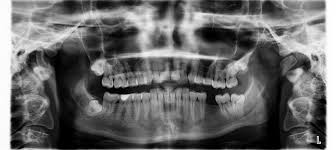
\includegraphics[width=\linewidth]{medical/mouth/0-gray.png}
    \caption{灰階原圖}
  \end{subfigure}
  \hfill
  \begin{subfigure}[t]{0.32\textwidth}
    \centering
    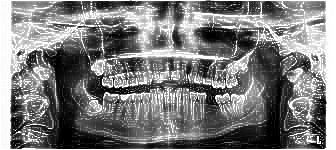
\includegraphics[width=\linewidth]{medical/mouth/4-sharpened.png}
    \caption{直接銳化}
  \end{subfigure}
  \hfill
  \begin{subfigure}[t]{0.32\textwidth}
    \centering
    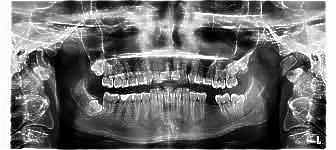
\includegraphics[width=\linewidth]{medical/mouth/6-denoised_sharpened.png}
    \caption{Mask 加回原圖}
  \end{subfigure}
  \caption{牙齒與下顎影像的原圖及兩種銳化結果比較。}
  \label{fig:mouth-sharpening}
\end{figure}

\subsection{頭骨影像}

\subsubsection{Laplacian 與 Gradient 比較}

如圖~\ref{fig:skull-laplacian-gradient}，Laplacian 整體較暗，
呈現頭骨內部的細碎紋理與較細的邊緣。
Gradient 的頭骨外框、眼眶及頸椎輪廓則較明亮、粗且連續，主要結構更容易辨認。
這與牙齒案例的趨勢相同：兩種運算對細碎變化與主要輪廓的呈現方式不同，
需依想觀察的細節選擇合適的結果。

\begin{figure}[H]
  \centering
  \begin{subfigure}[t]{0.48\textwidth}
    \centering
    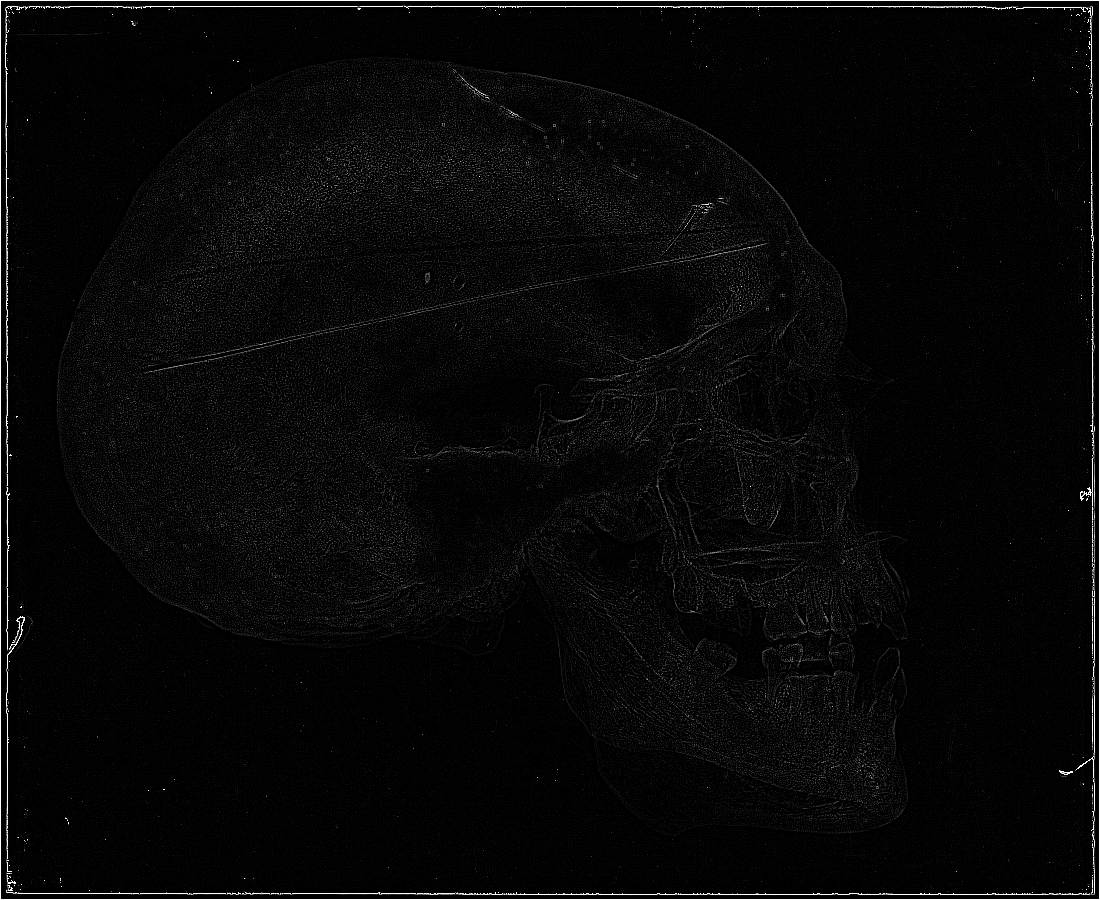
\includegraphics[width=\linewidth]{medical/skull/1-laplacian.png}
    \caption{Laplacian}
  \end{subfigure}
  \hfill
  \begin{subfigure}[t]{0.48\textwidth}
    \centering
    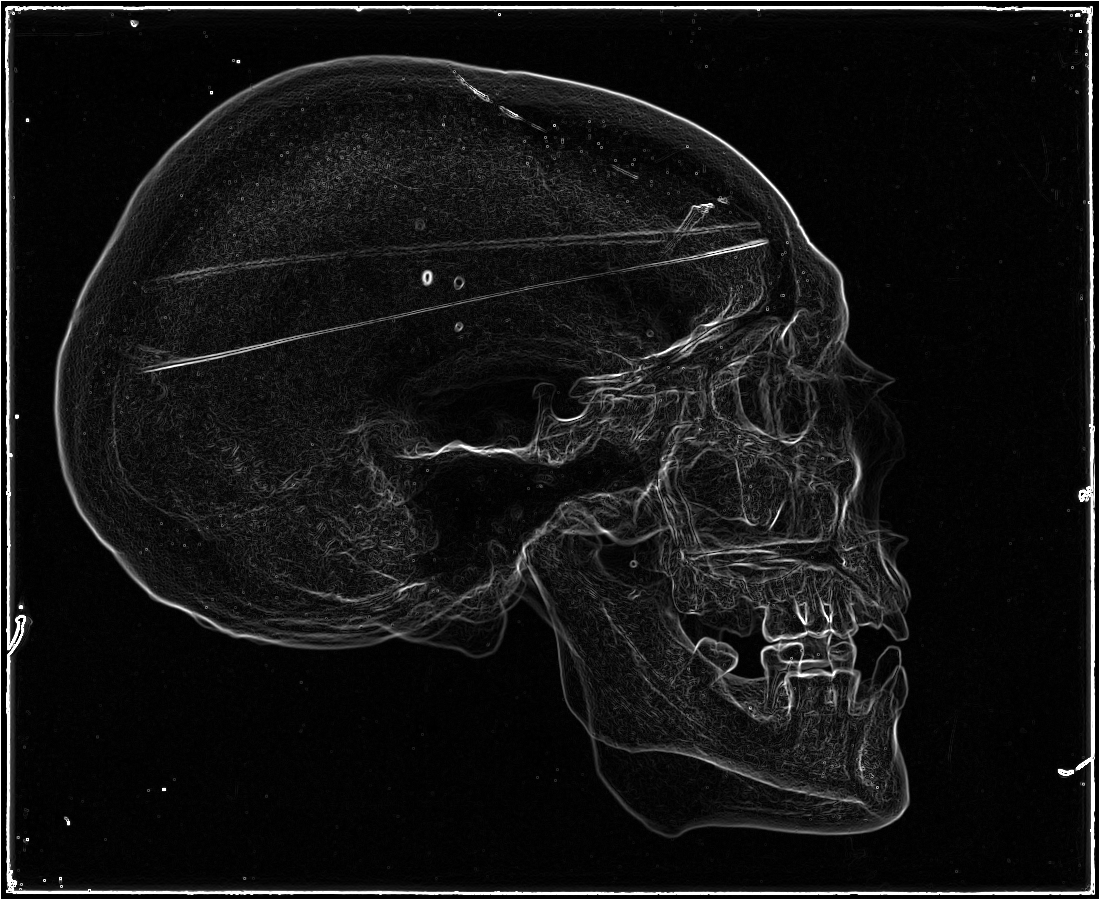
\includegraphics[width=\linewidth]{medical/skull/2-gradient.png}
    \caption{Sobel Gradient}
  \end{subfigure}
  \caption{頭骨影像的 Laplacian 與梯度大小比較。}
  \label{fig:skull-laplacian-gradient}
\end{figure}

\subsubsection{Laplacian 與 Mask 比較}

如圖~\ref{fig:skull-laplacian-mask}，相較於 Laplacian，
Mask 在頭骨內部的細碎反應較不明顯，整體更暗，
但頭骨外框與部分眼眶輪廓仍有保留。
這顯示乘上平滑梯度後，增強量較集中於梯度較明顯的位置。
另一方面，頭骨內部部分原本就較弱的細節也受到抑制，
因此不能僅以 Mask 的背景較暗，就認為所有細節都有改善。

\begin{figure}[H]
  \centering
  \begin{subfigure}[t]{0.48\textwidth}
    \centering
    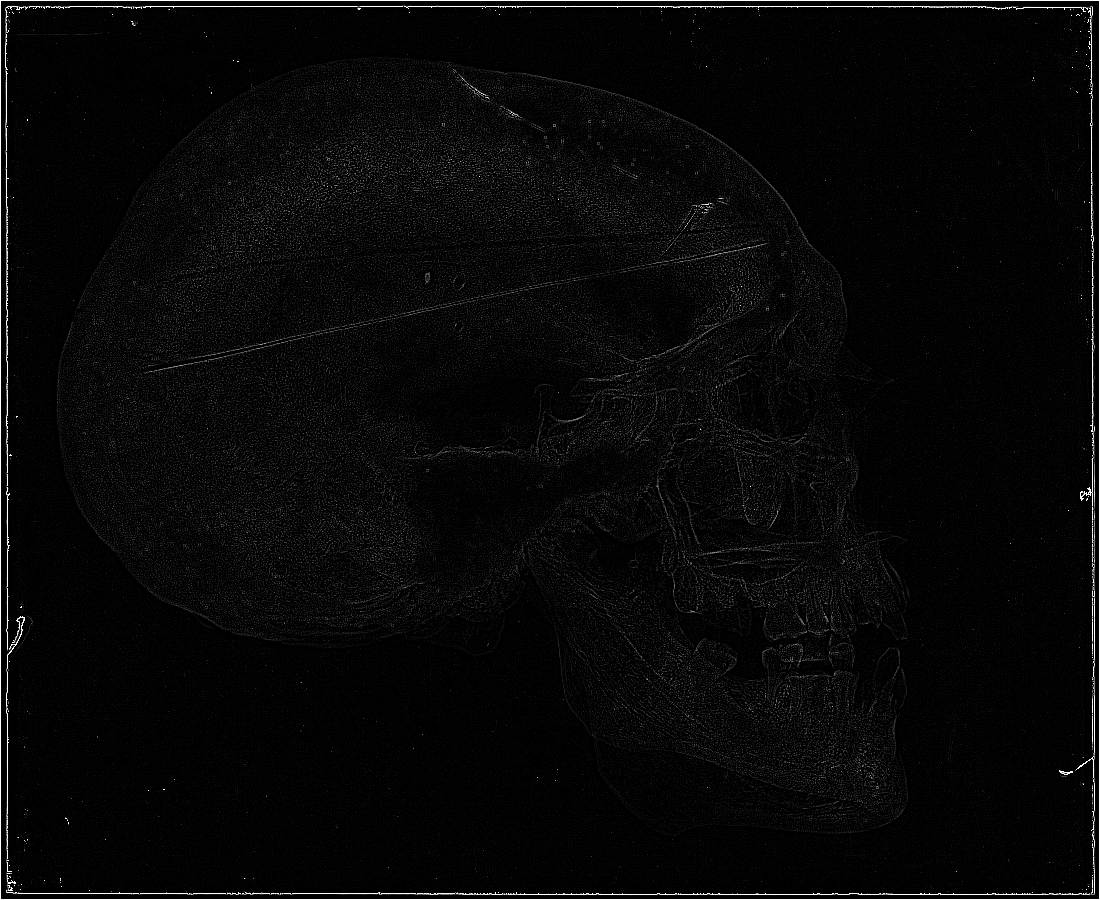
\includegraphics[width=\linewidth]{medical/skull/1-laplacian.png}
    \caption{Laplacian}
  \end{subfigure}
  \hfill
  \begin{subfigure}[t]{0.48\textwidth}
    \centering
    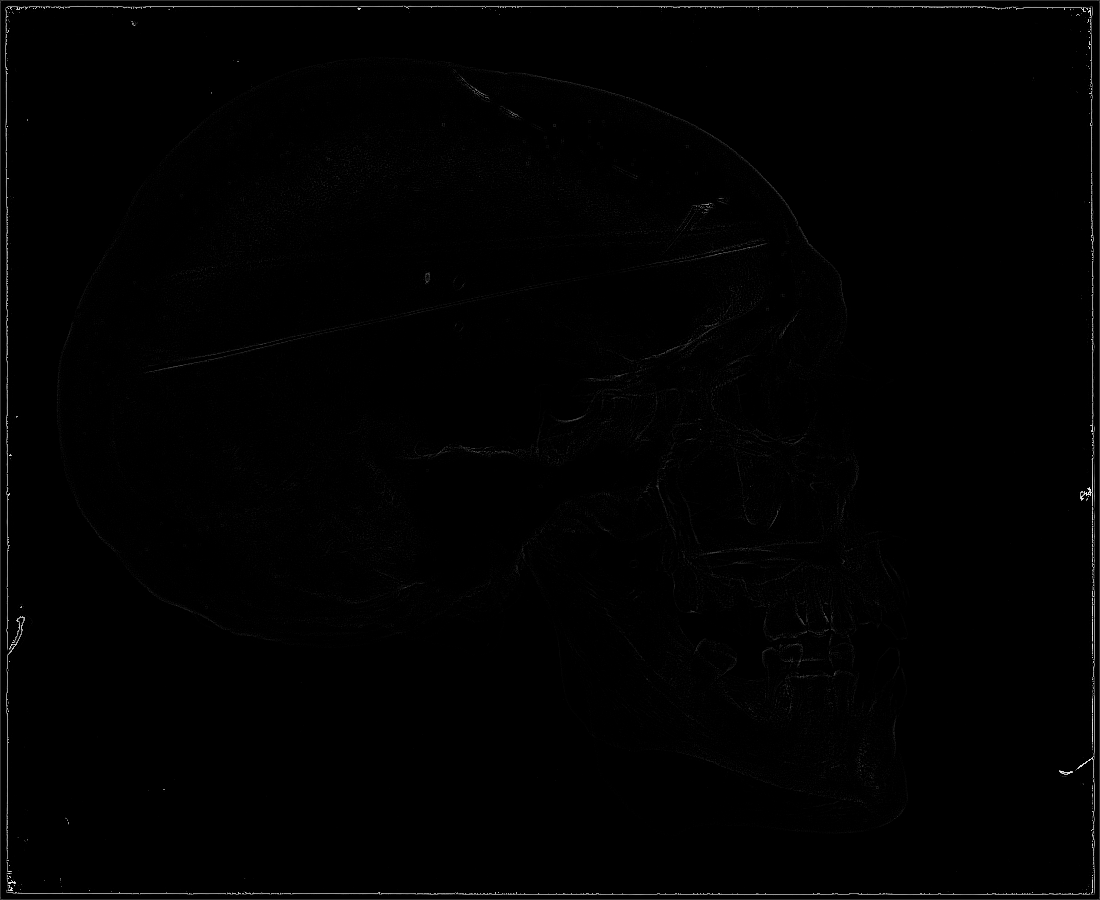
\includegraphics[width=\linewidth]{medical/skull/5-mask.png}
    \caption{Mask}
  \end{subfigure}
  \caption{頭骨影像的 Laplacian 與 Mask 比較。}
  \label{fig:skull-laplacian-mask}
\end{figure}

\subsubsection{原圖、Sharpened 與 Denoised Sharpened 比較}

如圖~\ref{fig:skull-sharpening}，相較於原圖，
直接銳化的 Sharpened 使頭骨外框與眼眶邊緣更明顯，
但頭骨上半部也出現較強的顆粒感與細碎紋理。
Denoised Sharpened 減弱了這些增強反應，保留主要輪廓，整體較接近原圖；
相對地，內部細節的增強程度也較小。
因此，使用 Mask 的效果可描述為降低直接銳化的部分細碎增強，
而細節保留的程度仍需配合影像內容評估。

\begin{figure}[H]
  \centering
  \begin{subfigure}[t]{0.32\textwidth}
    \centering
    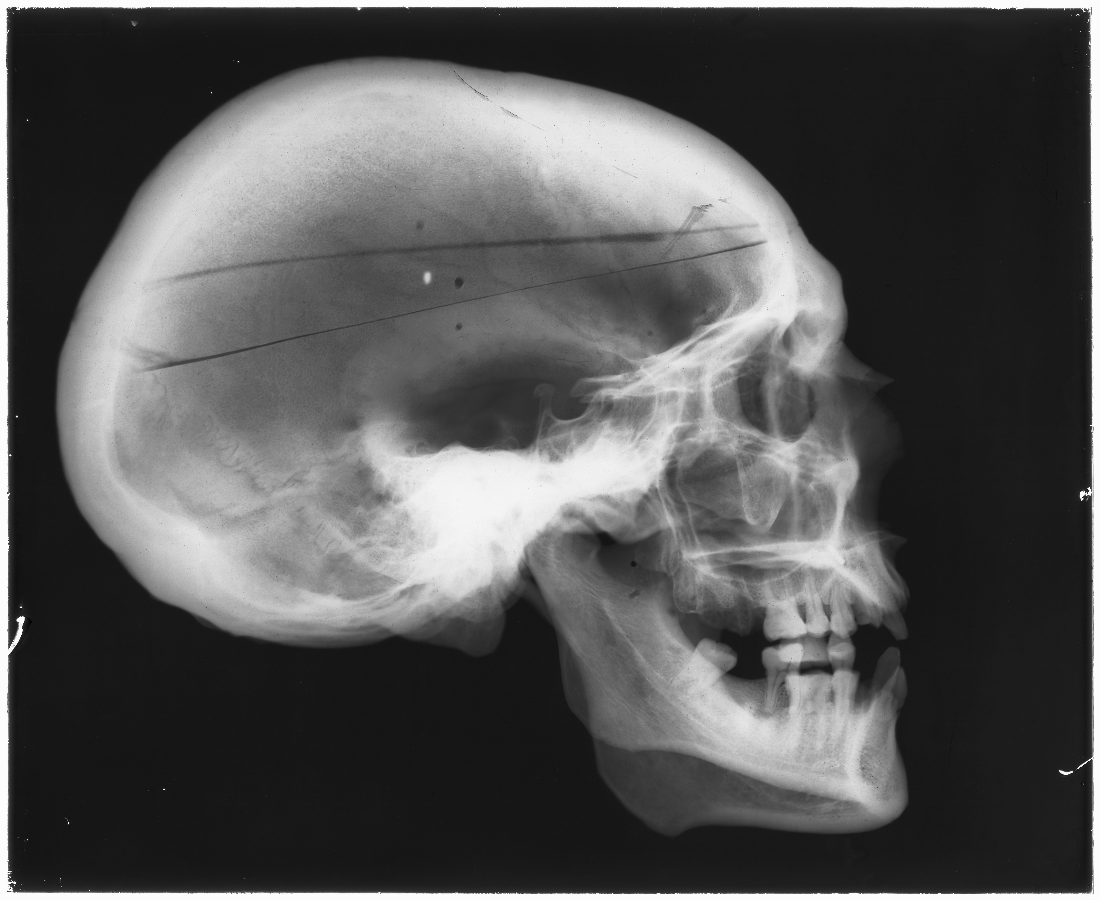
\includegraphics[width=\linewidth]{medical/skull/0-gray.png}
    \caption{灰階原圖}
  \end{subfigure}
  \hfill
  \begin{subfigure}[t]{0.32\textwidth}
    \centering
    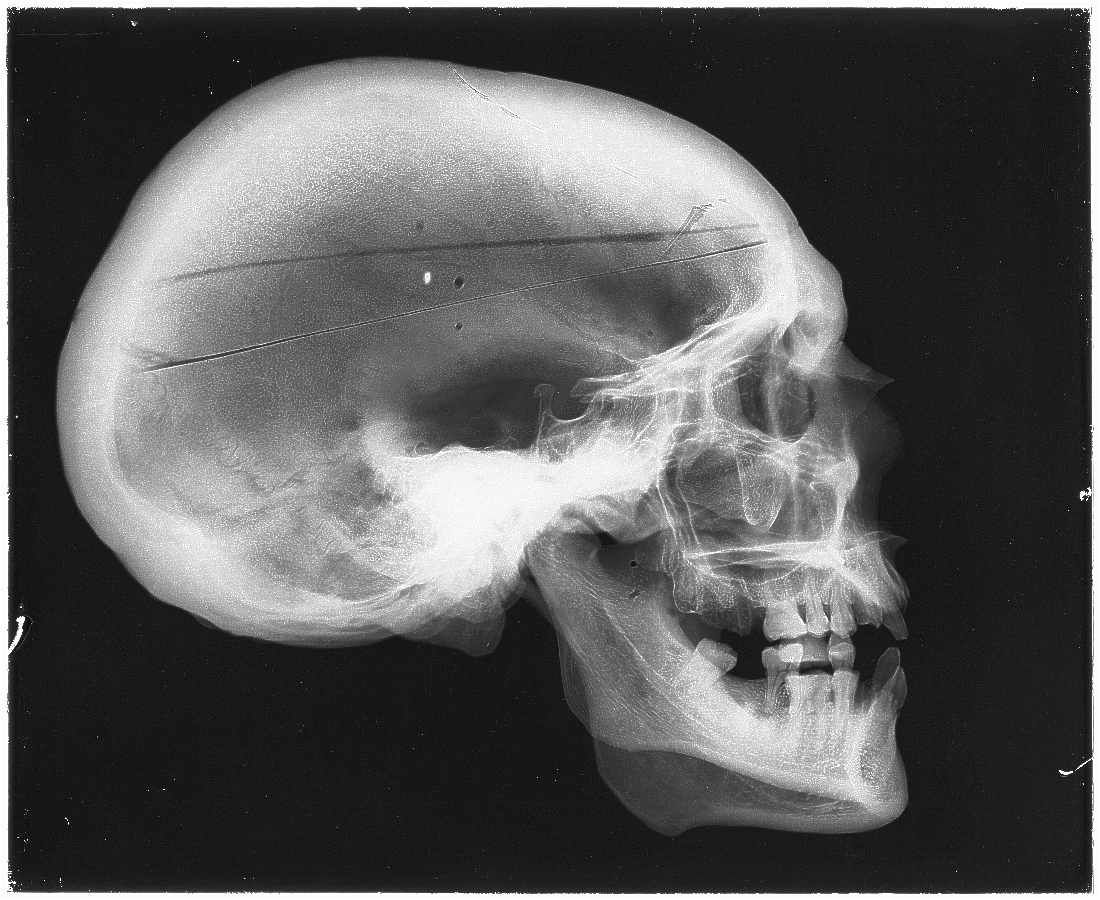
\includegraphics[width=\linewidth]{medical/skull/4-sharpened.png}
    \caption{直接銳化}
  \end{subfigure}
  \hfill
  \begin{subfigure}[t]{0.32\textwidth}
    \centering
    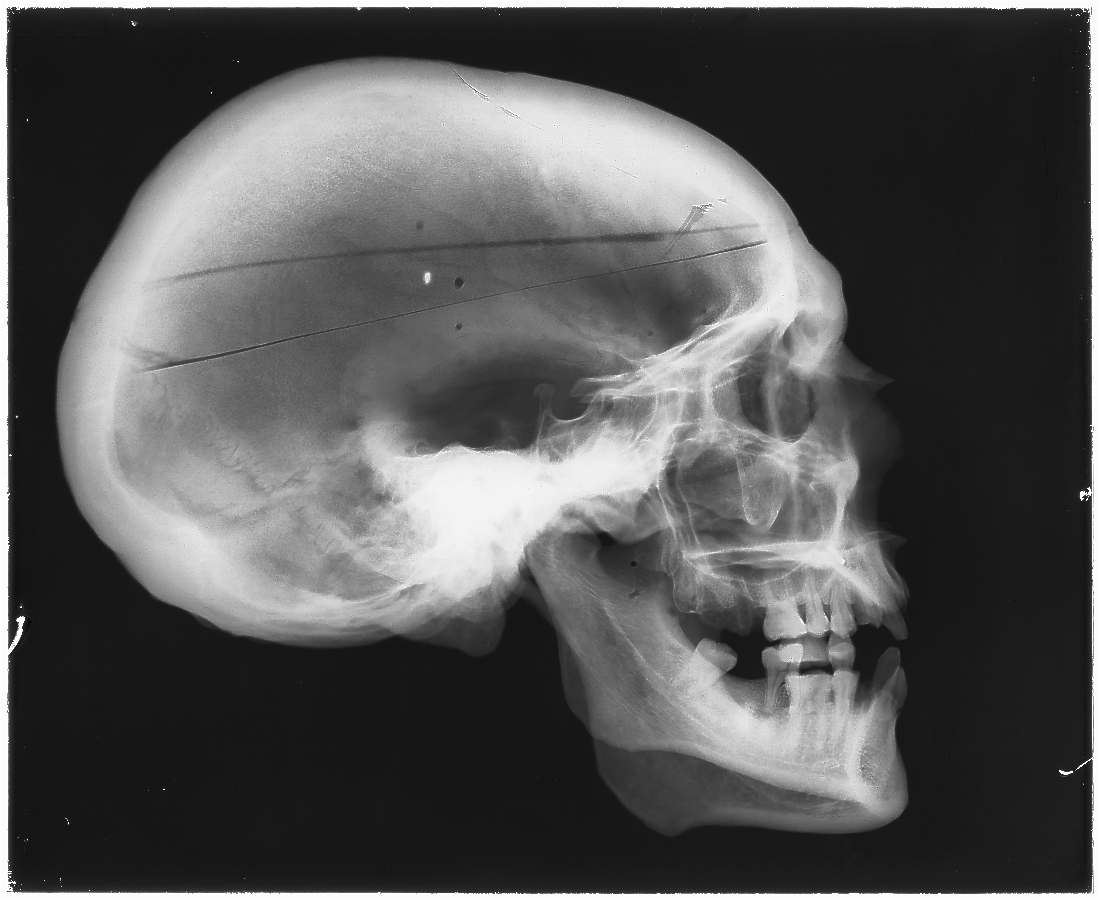
\includegraphics[width=\linewidth]{medical/skull/6-denoised_sharpened.png}
    \caption{Mask 加回原圖}
  \end{subfigure}
  \caption{頭骨影像的原圖及兩種銳化結果比較。}
  \label{fig:skull-sharpening}
\end{figure}

\subsection{兩個案例的共同觀察與限制}

兩個案例皆呈現相近趨勢：Laplacian 的細碎紋理與點狀反應較多，
Sobel Gradient 的主要輪廓較明顯；乘上平滑梯度後，Mask 的弱反應受到抑制。
將 Laplacian 直接加回原圖能強化邊緣，但也較容易增加顆粒與過強亮線；
改用 Mask 後，主要輪廓仍有保留，整體較接近原圖，但微小細節的增強量也較少。

程式將 Mask 銳化結果命名為 Denoised Sharpened。
本次圖片比較支持的是「相較於直接銳化，部分細碎增強反應減弱」，
尚未使用已知雜訊或無雜訊參考影像計算定量指標，因此降噪程度仍須額外驗證。
這些觀察也說明，銳化評估應同時考慮主要輪廓、微小紋理與顆粒感，
不能只依邊緣是否更亮判斷影像處理效果。

\medskip
\noindent\textbf{比較整理者：}待填。\quad
\textbf{實作者：}待填。\\
\textbf{審查者：}待填。\quad
\textbf{審查意見：}待實際檢查後填寫。

\clearpage
\section{卷積神經網路：自製模型與 PyTorch 比較}
\label{sec:cnn}

\subsection{實驗目的、資料與測試設定}

此題以 torch tensor 運算自行實作卷積、最大池化、Sigmoid 與前向傳遞，
再使用相同架構及參數的 PyTorch 模型作為對照，檢查兩者的輸出一致性。
本次實驗使用隨機初始化權重，觀察的是前向計算的數值結果；
這些輸出尚未透過訓練建立分類意義。

測試程式為 \texttt{test\_cnn.py}，模型定義位於 \texttt{cnn.py}。
在 \texttt{hw1} 資料夾執行下列指令，即可產生四組輸出、比較圖與摘要：

\begin{lstlisting}[language={},caption={CNN 比較實驗的執行指令}]
python test_cnn.py
\end{lstlisting}

表~\ref{tab:cnn-cases} 列出本次案例。
三張自製影像由程式繪製條紋、矩形與圓形，測試不同輸入大小；
照片案例讀取 \texttt{gamma\_normal.jpg}，以面積插值縮放為 $128\times128$。
輸入尺寸及輸出數量均落在題目指定範圍內。

\begin{table}[H]
  \centering
  \caption{CNN 測試案例與輸出設定。}
  \label{tab:cnn-cases}
  \begin{tabular}{@{}lccc@{}}
    \toprule
    案例 & 輸入影像（高、寬、通道） & 輸出向量 & Flatten 長度 \\
    \midrule
    \texttt{drawn-120} & $(120,120,3)$ & $3\times1$ & $7200$ \\
    \texttt{drawn-160} & $(160,160,3)$ & $5\times1$ & $12800$ \\
    \texttt{drawn-240} & $(240,240,3)$ & $10\times1$ & $28800$ \\
    \texttt{photo-128} & $(128,128,3)$ & $5\times1$ & $8192$ \\
    \bottomrule
  \end{tabular}
\end{table}

每組實驗設定 \texttt{torch.manual\_seed(7)}，輸入與模型參數皆使用
\texttt{float64}，在 CPU 上執行，並設定一個 torch 運算執行緒。
四組模型依輸入與輸出大小分別建立；同一組內的兩個模型才逐項複製參數並比較。

\begin{lstlisting}[caption={讀取或建立測試圖片，轉為模型輸入},label={lst:cnn-input}]
if name == 'photo-128':
    image = read_image(base / 'images' / 'gamma_normal.jpg')
    image = cv2.resize(image, (size, size), interpolation=cv2.INTER_AREA)
else:
    image = make_test_image(size)
height, width, channels = image.shape
rgb = cv2.cvtColor(image, cv2.COLOR_BGR2RGB)
x = torch.from_numpy(rgb.astype(np.float64) / 255.0)
x = x.permute(2, 0, 1).unsqueeze(0).contiguous()
\end{lstlisting}

程式~\ref{lst:cnn-input} 將 OpenCV 影像由 BGR 轉為 RGB，
把像素正規化至 $[0,1]$。
\texttt{permute} 將 $(H,W,C)$ 改排為 $(C,H,W)$，
\texttt{unsqueeze} 加入 batch 維度，得到 $(B,C,H,W)$，其中 $B=1$。
\texttt{contiguous} 使重排後的 tensor 具有連續的記憶體排列。

\subsection{網路架構與各層尺寸}

兩個模型皆使用兩組「卷積、Sigmoid、Max Pooling」，再接 Flatten、全連接層及 Sigmoid。
第一、第二個卷積層的輸出通道數分別為 $4$ 與 $8$；
核心大小均為 $3\times3$，stride 為 $1$、padding 為 $1$，因此卷積前後高寬相同。
最大池化使用 $2\times2$ 視窗及 stride $2$，每次使高寬減半。
最後的特徵長度為
\begin{equation}
  F=8\left\lfloor\frac{H}{4}\right\rfloor
       \left\lfloor\frac{W}{4}\right\rfloor.
  \label{eq:cnn-flatten}
\end{equation}
全連接層的權重形狀為 $(N,F)$，其中 $N$ 是該案例的輸出神經元數量。

\begin{table}[H]
  \centering
  \small
  \setlength{\tabcolsep}{3pt}
  \caption{四組案例的各層輸出尺寸；影像特徵依 $(B,C,H,W)$ 排列。}
  \label{tab:cnn-layer-shapes}
  \begin{tabular}{@{}lcccc@{}}
    \toprule
    階段 & \texttt{drawn-120} & \texttt{drawn-160} & \texttt{drawn-240} & \texttt{photo-128} \\
    \midrule
    Input & $(1,3,120,120)$ & $(1,3,160,160)$ & $(1,3,240,240)$ & $(1,3,128,128)$ \\
    Conv1 + Sigmoid & $(1,4,120,120)$ & $(1,4,160,160)$ & $(1,4,240,240)$ & $(1,4,128,128)$ \\
    Pool1 & $(1,4,60,60)$ & $(1,4,80,80)$ & $(1,4,120,120)$ & $(1,4,64,64)$ \\
    Conv2 + Sigmoid & $(1,8,60,60)$ & $(1,8,80,80)$ & $(1,8,120,120)$ & $(1,8,64,64)$ \\
    Pool2 & $(1,8,30,30)$ & $(1,8,40,40)$ & $(1,8,60,60)$ & $(1,8,32,32)$ \\
    Flatten & $(1,7200)$ & $(1,12800)$ & $(1,28800)$ & $(1,8192)$ \\
    FC + Sigmoid & $(1,3)$ & $(1,5)$ & $(1,10)$ & $(1,5)$ \\
    \bottomrule
  \end{tabular}
\end{table}

模型內部保留 batch 維度，所以最後的 tensor 為 $(1,N)$。
存檔時，程式先以 \texttt{reshape(-1,1)} 轉為 $N\times1$ 欄向量，
再分別輸出兩個模型的結果。
表~\ref{tab:cnn-layer-shapes} 的尺寸取自各組實際輸出的摘要檔。

\subsection{自製模型的程式實作}

\subsubsection{參數初始化}

\begin{lstlisting}[caption={自製 CNN 的參數初始化},label={lst:cnn-initialization}]
height, width, channels = input_size
output_count, _ = output_size
self.flatten_size = 8 * (height // 4) * (width // 4)
self.weight1 = torch.randn(4, channels, 3, 3, dtype=torch.float64) * 0.1
self.bias1 = torch.randn(4, dtype=torch.float64) * 0.1
self.weight2 = torch.randn(8, 4, 3, 3, dtype=torch.float64) * 0.1
self.bias2 = torch.randn(8, dtype=torch.float64) * 0.1
self.fc_weight = torch.randn(output_count, self.flatten_size,
                             dtype=torch.float64) / math.sqrt(self.flatten_size)
self.fc_bias = torch.randn(output_count, dtype=torch.float64) * 0.1
self.sigmoid = SigmoidActivation()
\end{lstlisting}

程式~\ref{lst:cnn-initialization} 為建構函式的核心參數設定，省略形狀紀錄等輔助程式。
卷積權重依「輸出通道、輸入通道、核心高、核心寬」排列，
每個輸出通道另有一個 bias。
卷積權重乘以 $0.1$，全連接權重依特徵長度縮放，
目的在控制初始加權和的尺度，降低 Sigmoid 大量落在接近 $0$ 或 $1$ 區域的機會。
全連接層依式~\eqref{eq:cnn-flatten} 的特徵數建立，確保各案例尺寸可銜接。

\subsubsection{自製卷積}

\begin{lstlisting}[caption={以 torch tensor 自行實作卷積},label={lst:cnn-convolution}]
def convolution(self, x, weight, bias, padding=1, stride=1):
    batch, channels, height, width = x.shape
    out_channels, _, kernel_h, kernel_w = weight.shape
    padded = x.new_zeros(batch, channels, height + 2 * padding,
                         width + 2 * padding)
    padded[:, :, padding:padding + height, padding:padding + width] = x
    out_h = (height + 2 * padding - kernel_h) // stride + 1
    out_w = (width + 2 * padding - kernel_w) // stride + 1
    out = x.new_zeros(batch, out_channels, out_h, out_w)
    for y in range(out_h):
        for col in range(out_w):
            region = padded[:, :, y * stride:y * stride + kernel_h,
                            col * stride:col * stride + kernel_w]
            products = region.unsqueeze(1) * weight.unsqueeze(0)
            out[:, :, y, col] = products.sum(dim=(2, 3, 4)) + bias
    return out
\end{lstlisting}

程式~\ref{lst:cnn-convolution} 先建立補零 tensor，再將原輸入放入中央區域。
兩層迴圈逐位置取出局部區塊，使用 broadcasting 同時計算各輸出通道，
對輸入通道與核心高寬加總後加入 bias。
batch 與輸出通道維度保持分開，輸出高寬則由核心、padding 與 stride 計算。
此函式使用 tensor 基本運算，自製模型未直接呼叫第三方卷積 API。

本 CNN 的核心直接與區塊逐項相乘，採用與對照模型相同的互相關規則，核心不旋轉。
前一節的空間濾波函式採數學卷積定義而先旋轉核心 $180$ 度；
這兩種介面各自依其比較目標定義，實驗時必須確認所採用的規則。

\subsubsection{自製最大池化與 Sigmoid}

\begin{lstlisting}[caption={自製最大池化},label={lst:cnn-pooling}]
def maxpool(self, x, pool_size, pool_stride):
    batch, channels, height, width = x.shape
    out_h = (height - pool_size) // pool_stride + 1
    out_w = (width - pool_size) // pool_stride + 1
    out = x.new_zeros(batch, channels, out_h, out_w)
    for y in range(out_h):
        for col in range(out_w):
            region = x[:, :, y * pool_stride:y * pool_stride + pool_size,
                       col * pool_stride:col * pool_stride + pool_size]
            out[:, :, y, col] = region.amax(dim=(2, 3))
    return out
\end{lstlisting}

程式~\ref{lst:cnn-pooling} 依池化視窗與 stride 取出區塊，
\texttt{amax(dim=(2,3))} 僅在空間維度取最大值，保留各 batch 與通道的獨立性。
本次視窗與 stride 都為 $2$，因此使用不重疊區塊，使高寬縮小。
自製模型使用此函式完成池化，未直接呼叫第三方 pooling API。

\begin{lstlisting}[caption={自行實作 Sigmoid},label={lst:cnn-sigmoid}]
class SigmoidActivation:
    def activate(self, z):
        return 1.0 / (1.0 + torch.exp(-z))
\end{lstlisting}

程式~\ref{lst:cnn-sigmoid} 將公式 $\sigma(z)=1/(1+e^{-z})$ 逐元素套用至 tensor。
本實驗在兩個卷積層及全連接層之後使用此函式。
輸出位於 $0$ 與 $1$ 之間，但其數值意義仍取決於模型的設定與訓練目的。

\subsubsection{自製前向傳遞}

\begin{lstlisting}[caption={自製 CNN 的前向傳遞},label={lst:cnn-custom-forward}]
def forward(self, x):
    out = self.convolution(x, self.weight1, self.bias1)
    out = self.sigmoid.activate(out)
    out = self.maxpool(out, 2, 2)
    out = self.convolution(out, self.weight2, self.bias2)
    out = self.sigmoid.activate(out)
    out = self.maxpool(out, 2, 2)
    out = out.reshape(out.shape[0], -1)
    out = out @ self.fc_weight.T + self.fc_bias
    return self.sigmoid.activate(out)
\end{lstlisting}

程式~\ref{lst:cnn-custom-forward} 依架構順序串接各操作。
\texttt{reshape} 保留 batch，將其餘特徵展平；
全連接層以矩陣乘法及 bias 計算加權和，最後再經過 Sigmoid。
程式片段省略了原程式中不影響結果的暫存變數賦值，運算順序相同。

\subsection{PyTorch 對照模型與相同權重比較}

\begin{lstlisting}[caption={PyTorch 對照模型},label={lst:cnn-pytorch}]
class ThirdPartyCNN(nn.Module):
    def __init__(self, input_size, output_size):
        super().__init__()
        height, width, channels = input_size
        output_count, _ = output_size
        self.conv1 = nn.Conv2d(channels, 4, 3, padding=1)
        self.conv2 = nn.Conv2d(4, 8, 3, padding=1)
        self.pool = nn.MaxPool2d(2, stride=2)
        self.flatten_size = 8 * (height // 4) * (width // 4)
        self.fc = nn.Linear(self.flatten_size, output_count)
        self.sigmoid = nn.Sigmoid()
        self.double()

    def forward(self, x):
        out = self.pool(self.sigmoid(self.conv1(x)))
        out = self.pool(self.sigmoid(self.conv2(out)))
        out = out.reshape(out.shape[0], -1)
        return self.sigmoid(self.fc(out))
\end{lstlisting}

程式~\ref{lst:cnn-pytorch} 使用 PyTorch API 建立相同的卷積、池化與全連接架構，
並以 \texttt{double()} 將浮點參數轉為雙精度，以配合輸入及自製模型。
前向傳遞中相鄰的呼叫以巢狀方式呈現，順序與原程式相同。
相同形狀只保證模型可銜接；為比較數值，還須將權重與 bias 完整複製。

\begin{lstlisting}[caption={建立模型、複製權重並計算兩組輸出},label={lst:cnn-copy-weights}]
torch.manual_seed(7)
custom = ConvolutionalNeuralNetwork((height, width, channels), output_size)
with torch.no_grad():
    custom_out = custom.forward(x)

third = ThirdPartyCNN((height, width, channels), output_size)
third.eval()
with torch.no_grad():
    third.conv1.weight.copy_(custom.weight1)
    third.conv1.bias.copy_(custom.bias1)
    third.conv2.weight.copy_(custom.weight2)
    third.conv2.bias.copy_(custom.bias2)
    third.fc.weight.copy_(custom.fc_weight)
    third.fc.bias.copy_(custom.fc_bias)
    third_out = third(x)
\end{lstlisting}

程式~\ref{lst:cnn-copy-weights} 將兩個卷積層及全連接層的六組參數逐項複製，
確保同組實驗使用相同輸入與相同參數。
固定隨機種子有助於重現初始化結果，而這裡實際的參數一致性由 \texttt{copy\_} 保證。
\texttt{no\_grad} 關閉梯度紀錄，適用於本次前向比較；
\texttt{eval} 將對照模型設定為評估模式。

\subsection{誤差定義與數值檢查}

對兩個模型的 $N$ 個輸出 $a_i$ 與 $b_i$，本實驗計算
\begin{align}
  \mathrm{MSE} &= \frac{1}{N}\sum_{i=1}^{N}(a_i-b_i)^2,
    \label{eq:cnn-mse}\\
  E_{\max} &= \max_{1\leq i\leq N}|a_i-b_i|.
    \label{eq:cnn-max-error}
\end{align}
MSE 用於描述平均平方差，最大絕對誤差則補充最不一致的一個輸出位置。

\begin{lstlisting}[caption={MSE 與輸出一致性檢查},label={lst:cnn-errors}]
def compare_outputs(custom, third):
    return torch.mean((custom - third) ** 2).item()

assert custom_out.shape == (1, output_count)
torch.testing.assert_close(custom_out, third_out, rtol=1e-9, atol=1e-10)
mse = compare_outputs(custom_out, third_out)
max_error = torch.max(torch.abs(custom_out - third_out)).item()
\end{lstlisting}

程式~\ref{lst:cnn-errors} 對逐元素差值平方後取平均，\texttt{item()} 將單一數值轉為 Python 數字。
程式另外檢查輸出形狀，並依指定的相對與絕對容許誤差比較兩個 tensor。
四組測試均通過這些檢查。

\begin{table}[H]
  \centering
  \caption{由本次摘要檔讀取的 CNN 輸出誤差。}
  \label{tab:cnn-errors}
  \begin{tabular}{@{}lcc@{}}
    \toprule
    案例 & MSE & 最大絕對誤差 \\
    \midrule
    \texttt{drawn-120} & $0$ & $0$ \\
    \texttt{drawn-160} & $1.232595\times10^{-32}$ & $2.220446\times10^{-16}$ \\
    \texttt{drawn-240} & $9.552613\times10^{-33}$ & $2.220446\times10^{-16}$ \\
    \texttt{photo-128} & $7.395571\times10^{-33}$ & $1.110223\times10^{-16}$ \\
    \bottomrule
  \end{tabular}
\end{table}

\subsection{測試圖片與輸出曲線比較}

\newcommand{\CNNCaseFigure}[3]{%
  \begin{figure}[H]
    \centering
    \begin{subfigure}[t]{0.30\textwidth}
      \centering
      \includegraphics[width=\linewidth]{cnn/#1-input.png}
      \caption{輸入影像}
    \end{subfigure}
    \hfill
    \begin{subfigure}[t]{0.66\textwidth}
      \centering
      \includegraphics[width=\linewidth]{cnn/#1-comparison.png}
      \caption{兩個模型的輸出}
    \end{subfigure}
    \caption{#2}
    \label{#3}
  \end{figure}%
}

圖~\ref{fig:cnn-drawn-120} 使用最小的 $120\times120$ 測試圖，輸出三個數值。
兩條曲線重疊，此次完整精度的輸出比較也得到 MSE 與最大絕對誤差皆為零。

\CNNCaseFigure{drawn-120}
  {自製幾何影像 \texttt{drawn-120}，輸出向量為 $3\times1$。}
  {fig:cnn-drawn-120}

圖~\ref{fig:cnn-drawn-160} 使用 $160\times160$ 影像，輸出五個數值。
兩條曲線在圖上仍重疊，完整精度下最大差異約為 $2.22\times10^{-16}$，
因此一般圖表尺度無法辨認此差異。

\CNNCaseFigure{drawn-160}
  {自製幾何影像 \texttt{drawn-160}，輸出向量為 $5\times1$。}
  {fig:cnn-drawn-160}

圖~\ref{fig:cnn-drawn-240} 測試題目輸入大小的上限，輸出十個數值。
Flatten 長度增加至 $28800$，兩個模型在較大的特徵尺寸下仍通過一致性檢查，
本組 MSE 約為 $9.55\times10^{-33}$。

\CNNCaseFigure{drawn-240}
  {自製幾何影像 \texttt{drawn-240}，輸出向量為 $10\times1$。}
  {fig:cnn-drawn-240}

圖~\ref{fig:cnn-photo-128} 改用實際照片，輸出五個數值。
兩個模型的曲線仍接近重疊，MSE 約為 $7.40\times10^{-33}$。
這組案例顯示在本次照片輸入條件下，自製運算與對照模型也得到接近一致的結果。

\CNNCaseFigure{photo-128}
  {實際照片 \texttt{photo-128}，輸出向量為 $5\times1$。}
  {fig:cnn-photo-128}

表~\ref{tab:cnn-photo-values} 列出照片案例儲存在 CSV 中的輸出，供數字對照。
數值保留至小數點後十五位；式~\eqref{eq:cnn-mse} 則使用格式化之前的原始
\texttt{float64} tensor 計算。
因此，表格中的末位差異不應直接當作完整精度下的實際誤差。

\begin{table}[H]
  \centering
  \small
  \caption{\texttt{photo-128} 的輸出數值（依 CSV 的十五位小數表示）。}
  \label{tab:cnn-photo-values}
  \begin{tabular}{@{}ccc@{}}
    \toprule
    輸出編號 & 自製模型 & PyTorch 模型 \\
    \midrule
    1 & \texttt{0.473947784342271} & \texttt{0.473947784342271} \\
    2 & \texttt{0.664193823150563} & \texttt{0.664193823150563} \\
    3 & \texttt{0.640714209828927} & \texttt{0.640714209828927} \\
    4 & \texttt{0.632176596193099} & \texttt{0.632176596193099} \\
    5 & \texttt{0.773140255311716} & \texttt{0.773140255311715} \\
    \bottomrule
  \end{tabular}
\end{table}

\subsection{結果討論與驗證範圍}

四組實驗涵蓋不同輸入尺寸、不同輸出數量及兩類影像內容，
MSE 為零或約 $10^{-32}$，最大絕對差異約 $10^{-16}$。
結果支持本次架構與測試條件下，自製前向計算與 PyTorch 對照模型的數值一致性。
極小的非零差異與雙精度浮點運算中不同加總順序的捨入差異相容，
不能將圖上重疊直接解讀為每個案例皆逐位元相同。

本次驗證的重點包括：正確的輸入維度、卷積與池化規則、Flatten 長度、
全連接運算，以及參數複製。
目前實驗使用 CPU、batch $1$、三通道方形影像與固定的網路架構；
對其他 batch、非方形輸入或不同核心設定的適用性，仍需另外測試。
權重由隨機數初始化，輸出曲線用來比較兩種計算流程，
其數值大小尚不能作為影像辨識能力的證據。

\medskip
\noindent\textbf{實作者：}待填。\quad
\textbf{審查者：}待填。\\
\textbf{審查意見：}待實際檢查後填寫。
